%%%%%%%%%%%%%%%%%%%%%%%%%%%%%%%%%%%%%%%%%%%%%%%%%%%%%%%
% Copied from previous \section{Neural Network Training}
A DNN-based binary classifier that distinguishes VBF signal from non-VBF signal events is used as a final discriminant in the VBF-enriched \TwoJet category.
%In the VBF-enriched \TwoJet category, a DNN-based binary classifier is used as a final discriminant.
This section describes how the DNN observable, also referred to as \emph{VBF DNN} in the following, is developed.\footnote{For this purpose, the author developed a software framework that makes use of industry-standard open-source ML libraries and manages the full ML cycle efficiently.
    The entire software suite used is summarized in \cref{app:dnn:software-suite}.
    It should also be noted that the training procedure has been modified several times during the course of the author's PhD, due to both improvements in the self-developed software and historical developments of the \HWW\ analysis (for example changes in MC simulated samples). If not mentioned otherwise, the results and procedures presented correspond to the final VBF DNN.}
The relevant supervised learning techniques are introduced in \cref{chap:ml}.
%The DNN is developed using simulated $pp$ collision events and is subsequently also applied to the data. 

\subsection{Methodology}
%Developing a neural network model for a physics analysis is a multi-stage and cyclic procedure.
The development of the VBF DNN can be described as a cyclic, multi-stage procedure:

\paragraph{Stage 1}
The first step is to prepare the training data.
The simulated samples that are listed in \cref{subsec:simulated-event-samples} are transformed in a way, so they can be easily used with state-of-the-art ML software. Details on the training data are given in \cref{subsec:training-data}

\paragraph{Stage 2}
The second stage is the main part of the DNN development and involves the training, validation, and optimization of the DNN.
This iterative workflow leads to the choice of input variables used in the DNN as well as choice of hyperparameters. This is presented in \cref{subsec:performance-metrics,subsec:hyper-parameters,subsec:input-variables-opt}.

\paragraph{Stage 3}
The third step is to deploy the neural network in the \HWW\ analysis, which includes the evaluation of data events with the DNN observable. Final measurement results based on the full statistical analysis that take into account all uncertainties can then be produced. This demonstrates the final performance of the trained DNN model, and reveals the weak-spots of the analysis and the developed model.
The latter information -- in particular information about what uncertainties dominate in the VBF, \HWW\ cross-section measurement -- can be used to adapt the training procedure in stage two and further improve the DNN model.
This also provides insights into how well the metric used to select a DNN model reflects the results from the statistical analysis.
%  to determine optimal training fractions. An example of such a study optimizing the EW $WW$ training fraction is discussed in \cref{app:sec:ewww-sample-fraction-optimization}.

\paragraph{Final model selection}
The final DNN model is selected when no further improvements can be made by repeating step two and three. It should be noted that the tasks involved in step three are time-consuming and computing-expensive, which limits the number of cycles that can realistically be carried out.
The validation of the final VBF DNN model can be found in \cref{subsec:fina-model-validation}. 

% that improvements of the self-developed software, together with historical developments of the entire \HWW\ analysis, lead to several modifications of the training setup over time. 

% During the course of the author's doctoral studies, some approaches have evolved, which means that certain parts of the training procedure have been optimized based on earlier versions of the training setup than the version used for the final DNN. 
% The following outlines roughly the different stages of the training, to motivate the procedures and decisions that were taken that resulted in the development of the final DNN used in this analysis. 
% The hyperparameters and procedure used for the final DNN are summarized in \cref{tab:hyper-parameters}.

%%%%%%%%%%%%%
% DISTINGUISH??: Physics based optimization, DNN based, empirical optimization

% - Historical developments, features freezes, limitations of computing resources/turnaround time
% The following therefore is an attempt to only a rough outline of the different stages of the training, which, due to both historical developments and the empirical nature of ML, should not be taken at face value but rather viewed as an attempt to roughly describe the approaches and procedures that have led to the development of the final DNN. 


\subsection{Training data and data preparation}
\label{subsec:training-data}
All MC simulated events that pass the preselection (see \cref{subsec:preselection}) and satisfy $\TwoJet$ are used for the training. To increase the amount of sample events with which the DNN is trained, no other VBF-specific selections are applied prior to the training. This has proven to be particularly beneficial in the development of DNNs, which perform better the larger the dataset available for the training.
%This increases the size of the training data 
%This has proven advantageous compared to a training using, for example, only events in the VBF-enriched \TwoJet category. 
The size of the available training samples are shown in \cref{tab:DNNtrainingstats} along with other specifications that are discussed below.
\begin{table}[ht]
    \centering
    \small
    \begin{tabular}{ c  | r c c c}
        \toprule
        Background sample  & Raw events & Label & $S_\text{frac}$ \\
        \midrule
        % $H_{\mathrm{VBF}}$ & 390195     & 1     & 0.05            \\
        % $H_{\mathrm{ggF}}$ & 115185     & 0     & 0.05            \\
        % $t\bar{t}$         & 997679    & 0     & 0.4             \\
        % $Wt$               & 997679      & 0     & 0.07            \\
        % $WW$ (Strong)      & 1723237    & 0     & 0.2             \\
        % $WW$ (EW)          & 997679     & 0     & 0.12            \\
        % $Z/\gamma*$        & 997679     & 0     & 0.2             \\
        % $V\gamma$          & 12585       & 0     & 0.01            \\
        % Other $VV$         & 997679     & 0     & 0.02            \\
        $H_{\mathrm{VBF}}$ & 390000     & 1     & 0.05            \\
        $H_{\mathrm{ggF}}$ & 120000     & 0     & 0.05            \\
        $t\bar{t}$         & 1530000    & 0     & 0.4             \\
        $Wt$               & 60000      & 0     & 0.07            \\
        $WW$ (Strong)      & 1900000    & 0     & 0.2             \\
        $WW$ (EW)          & 220000     & 0     & 0.12            \\
        $Z/\gamma*$        & 1000000    & 0     & 0.2             \\
        $V\gamma$          & 13000      & 0     & 0.01            \\
        Other $VV$         & 680000     & 0     & 0.02            \\
        \bottomrule
    \end{tabular}
    \caption{Specification of the training data used for the development of the VBF DNN. The raw events correspond to the number of generated events, disregarding any weight. More information on the training fraction $S_\text{frac}$ is given in the text.}
    \label{tab:DNNtrainingstats}
\end{table}
The training events are labelled with \emph{target} labels $t_n$ to distinguish VBF signal events ($t_n = 1$) from all other types of processes ($t_n = 0$).
The ggF signal is treated like all other backgrounds, so it is implicitly referred to when ``backgrounds'' are mentioned in this section.
Events with misidentified leptons are not considered in the training because of the complex data-driven procedure that is used to estimate their contribution.
Prior to the training, the training data are shuffled, and the input variables standardized to have a mean of 0 and a standard deviation of 1.
Each training event gets assigned a \emph{training weight}, $w_\text{train}$, that is used in the calculation of the loss function. It is determined by the product of two other weights,
\begin{equation}
    w_\text{train} = w_\text{phys} \times w_\text{proc}.
\end{equation}
% process_weight = total_phys_weight * fraction / total_sample_phys_weight
% fraction = sum(training weight sample) / total sum training weight
The \emph{physical weight}, $w_\text{phys}$, normalizes the events according to their theoretical cross-section predictions, and the \emph{process weight}, $w_\text{proc}$, is defined per process in order to control the importance given to a specific process in the training.
%The latter weight allows controlling the importance given to a specific event sample in the training. 
The latter weight is determined by specifying a desired \emph{training fraction}, $S_\text{frac}$, which can be considered as the fractional contribution to the loss function of a particular process $p$,
\begin{equation}
    S_\text{frac} = w_\text{proc} \frac{\sum_{p} w_\text{phys}}{ \sum w_\text{phys}},
\end{equation}
where the sum in the numerator goes over all events of process $p$, and the sum in the denominator over the entire training data. The training fraction provides a meaningful way to encode the importance of different processes and to remove sample imbalances in the training data. They have been optimized as explained below.
% The chosen values for the final VBF DNN are shown in \cref{tab:DNNtrainingstats}.
% They have been optimized as discussed in \cref{}.
% Taking into account both the physical weights and the process weights, the \emph{training training fraction} is defined as the fractional contribution of a given sample to the loss function calculation.
%Prior to the training, the training data are shuffled and categorized into different folds according to the number of folds $k$ specified. 
%The network is then trained according to the specified number of folds $k$. 

\subsection{Training procedure and DNN discriminant}
\label{subsec:performance-metrics}
%%%%%%%%%%%%%%%%%%%%%%%%%%%%%%%%%%%
% Performance metric explanation
The VBF DNN is trained using the $k$-fold cross validation method with $k=5$ and the training data split as explained in \cref{subsec:par:kfold-crossval}.
The validation set is used to compare the performance of different trainings, for example, to optimize the set of hyperparameters.
The distribution of the DNN output for the validation set is shown in \cref{fig:dnn-val-set-a}.
\begin{figure}[ht]
    \subfloat[] {
        \newImageResizeCustom{0.47}{figures/hww/dnn/CutVBF_SR_reTrained_default_40bins.pdf}
        \label{fig:dnn-val-set-a}
    }
    \subfloat[] {
        \newImageResizeCustom{0.47}{figures/hww/dnn/CutVBF_SR_reTrained_default_optBinning_zoom.pdf}
        \label{fig:dnn-val-set-b}
    }
    \caption{DNN output distribution for the validation set of the training data for (a) the full range of DNN output values and an equidistant binning and (b) the range [0.6-1.0] with high VBF signal purity and a binning chosen to mitigate the effects of statistical fluctuations. Details on the binning as well as the significance metric are provided in the text.}
    \label{fig:dnn-val-set}
\end{figure}
As can be seen, the VBF signal purity improves as the DNN output value increases.
Significance-based performance metrics that determine the excess of VBF signal events over background events are used to compare different trainings and choose optimal hyperparameters.
The significance metric is evaluated according to
\begin{equation}
    \label{eq:significance-performance-metric}
    Z0 = \sqrt{ \sum_{i \in \text{bins}} Z(s_{i}, b_{i}, \sigma_{i})^2 },
\end{equation}
where the sum goes over all bins of the histogram, and $Z$ is defined as in \cref{eq:simple-sign}.
The value of this metric is largely driven by the bins with the largest signal purity, in particular the highest bin.
To mitigate the effect of statistical fluctuations, as well as to allow for fair comparisons between DNN models that have different shapes, the histogram of the DNN output is rebinned. The binning is chosen as in the statistical analysis which is explained in \cref{subsec:fina-model-validation}. \Cref{fig:dnn-val-set-b} shows the rebinned DNN output distribution in the region where the VBF signal is most dominant. 
%The $Z0$ values corresponding to the distributions shown with equidistant (modified) binning are 9.9 (9.6).
%\todo{Point to binning algorithm}
% It corresponds to the square root of the sum of the squared significances calculated in each of the histogram bins according to \cref{eq:simple-sign}.
% PERFORMANCE METRICS
% Three different performance metrics based on \cref{eq:significance-performance-metric} are therefore considered:
% \begin{enumerate}
%     \item $Z0$(40 bins): uses a histogram with 40 equidistant bins.
%     \item $Z0$(var. bins): uses a histogram with variable sized bins determined by taking into account the number of signal and background events as well as the relative background uncertainty. This is described in \todo{reference to section} \cref{subsec:statistical-model}. This allows a fair comparison between different neural network models, in particular if they have different shapes.
%     \item $Z0$(var. bins + syst. unc.): uses the same histogram as $Z0$(var. bins) and in addition takes into account approximate, process-specific systematic uncertainties, $\sigma_{\text{approx}}^\text{rel}$, in the calculation of $Z_{i}(s, b, \sigma)$ in \cref{eq:significance-performance-metric}. The uncertainties are taken from a previous iteration of the analysis and reflect relative uncertainties of the expected number of events, $n_p$, in the highest DNN bin. They are specified in \cref{tab:DNNtrainingstats}. The final value of $\sigma$ is determined by $\sigma = \sqrt{ \sum_{p \in \text{processes}} \left( n_p * \sigma_\text{approx, p}^\text{rel} \right)^2}$.
% \end{enumerate}

The test set of the cross-validation split is used to deploy the model in the analysis as well as for tests of generalization.
\Cref{fig:dnn-train-vs-test} shows comparison plots between the training and the test set, confirming good agreement between the two and thus ruling out the occurrence of severe overfitting.\footnote{It is worth noting that even if some overfitting occured, it would not introduce any errors or biases in the analysis, since the test set of the cross-validation method is used to evaluate the simulated samples in the final analysis. It would merely indicate that the DNN trained is not the most optimal discriminant.}
The distributions also nicely visualize the different shapes of the VBF signal and the backgrounds.
The VBF DNN distribution as used in the statistical analysis can be found in \cref{subsec:fina-model-validation}
% Model choice: Choose model with highest significance in validation set!
% Model validation: Validate model comparing against test set!
\captionsetup[subfloat]{captionskip=7pt} % space between subfloat caption and image
% Plots made with SFUsMLKit on cedar with:
% ./plot.py -c configs/HWW/winningSubmission.cfg --trainingFolderName dropout-02-5-fold-aggressive-lr-schedule-2-fine-scan-ewww-scan-etafix/210805_9_0.12_8226149877761426764


\begin{figure}[t]
    \subfloat[] {
        \newImageResizeCustom{0.49}{figures/hww/dnn/train_vs_test_dnn_score_normalized_log.pdf}
    }
    \subfloat[] {
        \newImageResizeCustom{0.49}{figures/hww/dnn/train_vs_test_dnn_score_zoom_non-normalized_non-log.pdf}
    }
    \caption{Comparison of the DNN output distributions for the training set and test set of the training data for (a) the full range of DNN output values and (b) the region with high VBF signal purity.}
    \label{fig:dnn-train-vs-test}
\end{figure}


\subsection{Choice of hyperparameters}
\label{subsec:hyper-parameters}
% The optimization problem is multi-dimensional, which means that, for example, optimising a parameter $B$ after optimising parameter $A$ may result in the value of parameter $A$ no longer being optimal.
% Choosing and optimizing a set of hyperparameters for the DNN training is a vastly empirical procedure.
% While some parameters are crucial for a successful training, such as the learning rate, others show little impact on the results and rely on simple choices.
The complete set of hyperparameters chosen for the final VBF DNN training is summarized in \cref{tab:DNN-info}. The model architecture used is a feedforward DNN with one output layer and a logistic sigmoid as activation function. All other nodes use the ReLU activation function.
The performance of different architectures with different number of layers and nodes was studied and are presented in \cref{app:dnn:opt-studies}.
The model chosen has 7 hidden layers with decreasing number of nodes, specifically {256, 128, 64, 32, 24, 16, 8}.
%, which amounts to a total number of weights of $\mathcal{O}$(10k). 

\begin{table}[t]
    \begin{center}
        
\begin{tabular}{l l}
    \toprule
    Parameter/Characteristic & Value \\
    \midrule
    Input layers & 15 \\ 
    \multirow{2}{*}{Input variables}  & \mjj, \dyjj, \lepetacent, \mlonejone, \mlonejtwo, \mltwojone, \mltwojtwo, \\
    & \pTjone, \pTjtwo, \pTjthree, \dphill, \mll, \mT, \pttot, \METSig\\ 
    Hidden layers & {256, 128, 64, 32, 24, 16, 8} \\
    Activation & ReLU \\ 
    Output layers & 1 \\
    Output activation & sigmoid \\ 
    Loss function & cross-entropy \\ 
    Learning rate & 9 \\
    Batchsize & 512 \\ 
    Optimizer & AdaGrad \\
    Dropout &  20\% \\ 
    Epochs & 40 \\
    Training weights & optimized \\ 
    Training sets/folds & 5 folds (train/val/test) \\
    \bottomrule
\end{tabular}

    \end{center}
    \caption{Hyperparameters and training methods used for the development of the final VBF DNN.
    }
    \label{tab:DNN-info}
    % Nominal values, statistical uncertainties and EWSUBTR uncertainties produced on tag kon_improveZjetsFFStats_v2
\end{table}

During the training, dropout is used as regularization by randomly disabling 20\% of weights in each weight update cycle.
The batchsize is chosen to be 512, which is a tradeoff between granularity and training time.
The cross-entropy loss is used as loss function and takes into account the training weights.
\Cref{fig:monitoring} shows the loss and binary accuracy\footnote{The binary accuracy is defined by counting a VBF signal event (non-VBF signal event) as correctly classified if the DNN output value is larger (smaller) 0.5.
} evaluated during the training with the validation set.
The curves shown look as expected from a well converging training with a suitable set of hyperparameters and no sign of overfitting\footnote{Overfitting would be reflected in a diverging validation loss after a certain epoch.} is observed. These metrics are not used for comparing the performance of different trainings, but are useful measures to validate the training settings. For all studies conducted, different learning rates are tested and the optimal value chosen.
For the training of the VBF DNN the learning rate is set to 9.
The performance of different optimizers was also studied and showed very comparable results. The AdaGrad optimizer is chosen for the training of the VBF DNN.

The training fractions used in the training are indicated in \cref{tab:DNNtrainingstats}. They were chosen to approximate the relative theoretical cross-section normalization between the samples at preselection, with some exceptions: The VBF signal training fraction is increased to 5\% because it is the main target of the training. Increasing this fraction further did not show any improvements. Furthermore, the training fractions of the ggF and EW $WW$ samples are increased compared to their cross-section normalization. This is done to take into account their large relative contributions in the VBF-like phase space despite their low overall normalization. The study conducted to choose the EW $WW$ weight is presented in \cref{app:sec:ewww-sample-fraction-optimization}.

\begin{figure}[t]
    \subfloat[] {
        \newImageResizeCustom{0.47}{figures/hww/dnn/loss_thesis.pdf}
    }
    \subfloat[] {
        \newImageResizeCustom{0.47}{figures/hww/dnn/accuracy_thesis.pdf}
    }
    \caption{(a) Cross-entropy loss and (b) binary accuracy evaluated for both the training set and validation set as a function of training epochs. The metrics are averaged over five different trainings, with the shaded band corresponding to the standard deviation.}
    \label{fig:monitoring}
\end{figure}


\subsection{Choice and validation of input variables}
\label{subsec:input-variables-opt}
The greatest impact on the performance of the VBF DNN have the type and number of input features used.
Several sets of observables were studied for use as DNN input variables which is summarized in \cref{app:dnn:opt-studies}.
The one with the highest significance metric $Z0$(var. bins) as evaluated on the validation set is chosen, and corresponds to a set of in total 15 variables.
Their distributions are shown in \cref{fig:dnn-inputs-post-fit1,fig:dnn-inputs-post-fit2}.
They exploit various features of the VBF signal process (see \cref{subsec:signal-bkg-characterisation}) that can be grouped into three categories:

\paragraph{VBF topology}
A set of 10 of the 15 input variables target the distinct VBF topology: \mjj, \dyjj, and the sum of the lepton centralities, \lepetacent, show clear discrimination power against the background processes (see \cref{fig:dnn-inputs-post-fit-1,fig:dnn-inputs-post-fit-2,fig:dnn-inputs-post-fit-3}). More subtle differences between the VBF signal and the background distributions can be seen for the invariant masses of all four possible lepton-jet pairs between the leptons and the two leading jets (\mlonejone, \mlonejtwo, \mltwojone, \mltwojtwo). These observables take on average slightly larger values for the VBF signal (\cref{fig:dnn-inputs-post-fit-4,fig:dnn-inputs-post-fit-5,fig:dnn-inputs-post-fit-6,fig:dnn-inputs-post-fit-7}), especially when compared to \ttbar processes where two of the lepton-jet combinations have an upper threshold of 173\,\GeV, assuming that the jets originate from the top-quark decays.
The \pT of the three leading jets (\pTjone, \pTjtwo,\pTjthree, where \pTjthree is set to 0 if there is no third jet present in the event) provide additional discrimination.
Because of the two high-energy jets expected in the VBF production, the VBF signal causes slightly larger \pTjone and \pTjtwo values than the background processes (\cref{fig:dnn-inputs-post-fit-8,fig:dnn-inputs-post-fit-9}).
The \pTjthree observable takes on average smaller values for the VBF signal (\cref{fig:dnn-inputs-post-fit-10}) because of the small hadronic activity in the rapidity gap spanned by the jets. The \pTjthree variable is particularly meaningful because it is the only observable that provides information about whether a third jet is present.

\captionsetup[subfloat]{captionskip=5pt} % space between subfloat caption and image
\begin{figure}[ht]
    \centering
    \subfloat[$\mjj$]{
        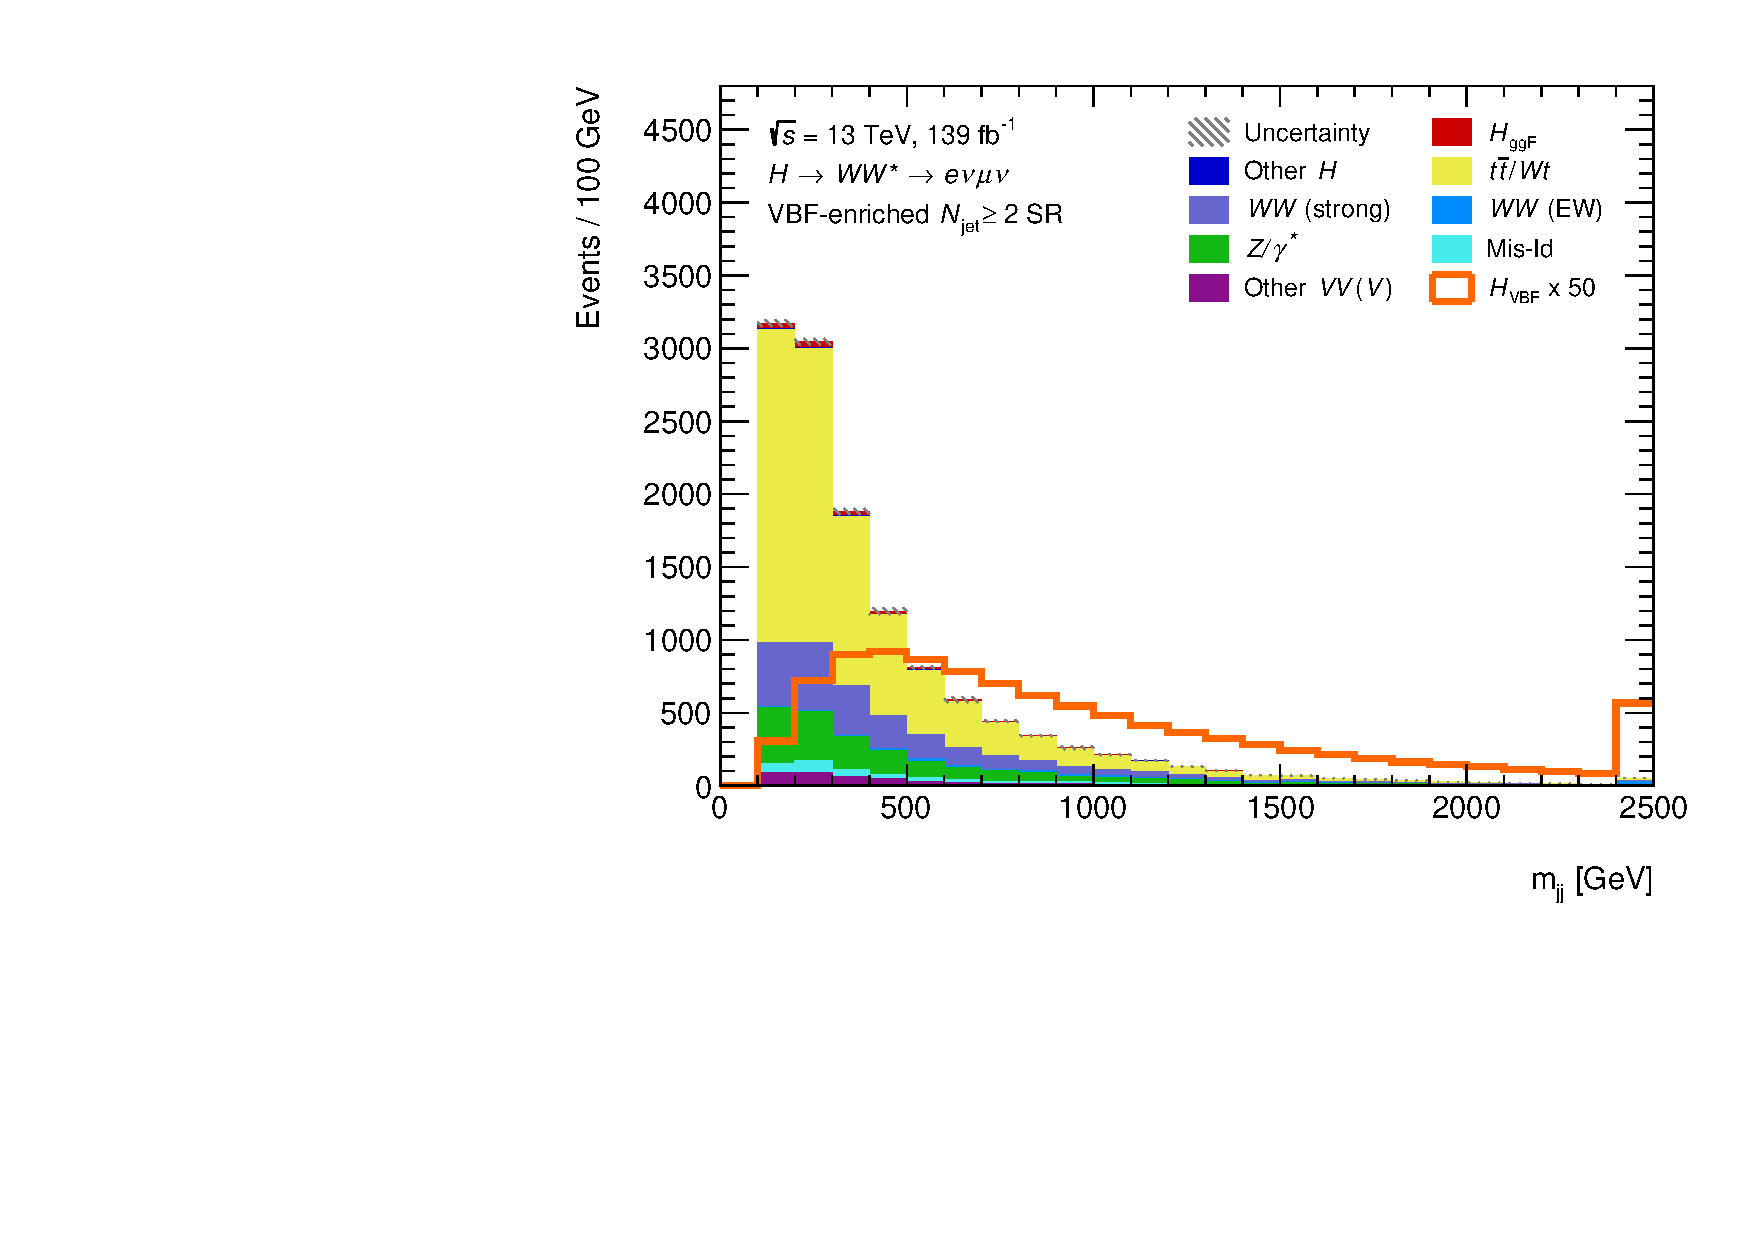
\includegraphics[width=0.32\textwidth]{figures/hww/dnn/blinded/run2-emme-CutVBF_SR-Mjj-lin.pdf} \hfill
        \label{fig:dnn-inputs-post-fit-1}
    }
    \subfloat[$\dyjj$]{
        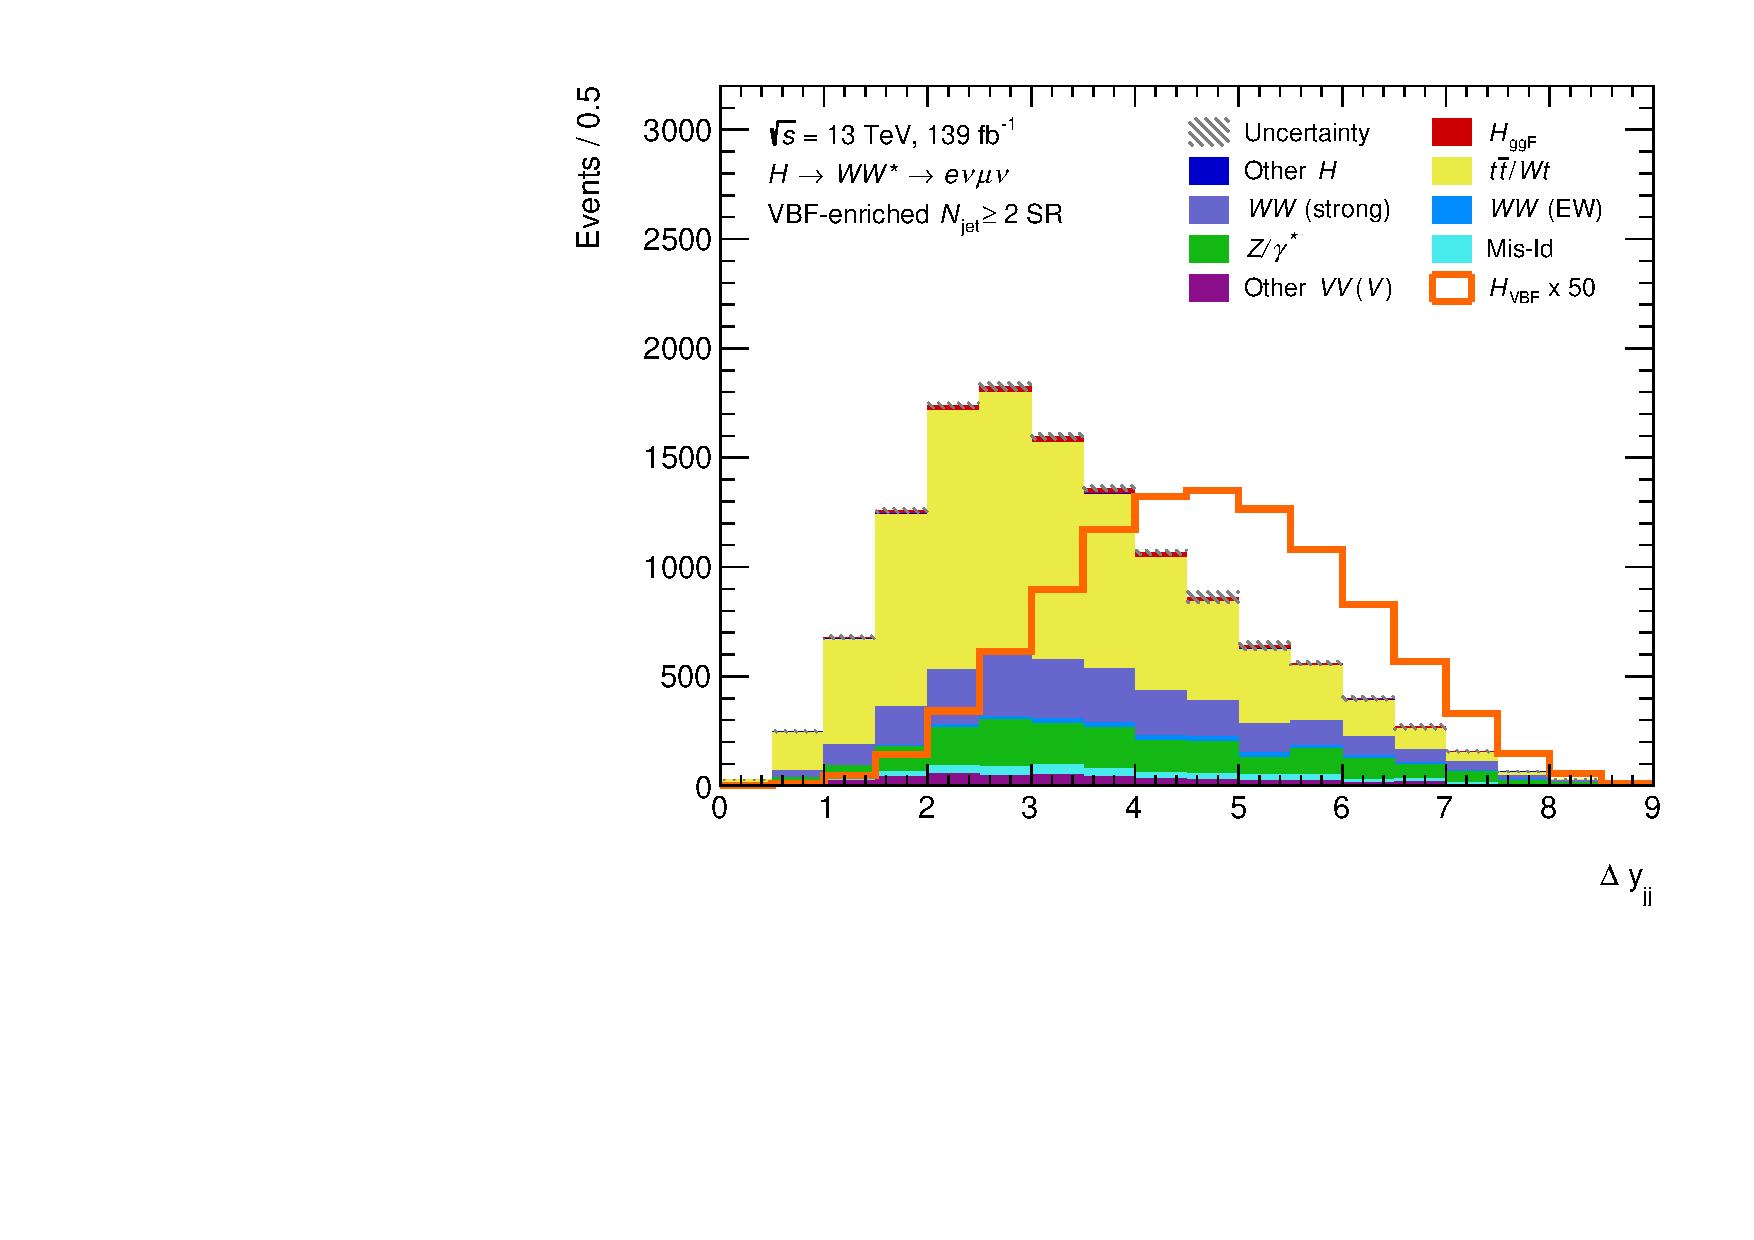
\includegraphics[width=0.32\textwidth]{figures/hww/dnn/blinded/run2-emme-CutVBF_SR-DYjj-lin.pdf} \hfill
        \label{fig:dnn-inputs-post-fit-2}
    }
    \subfloat[$\lepetacent$]{
        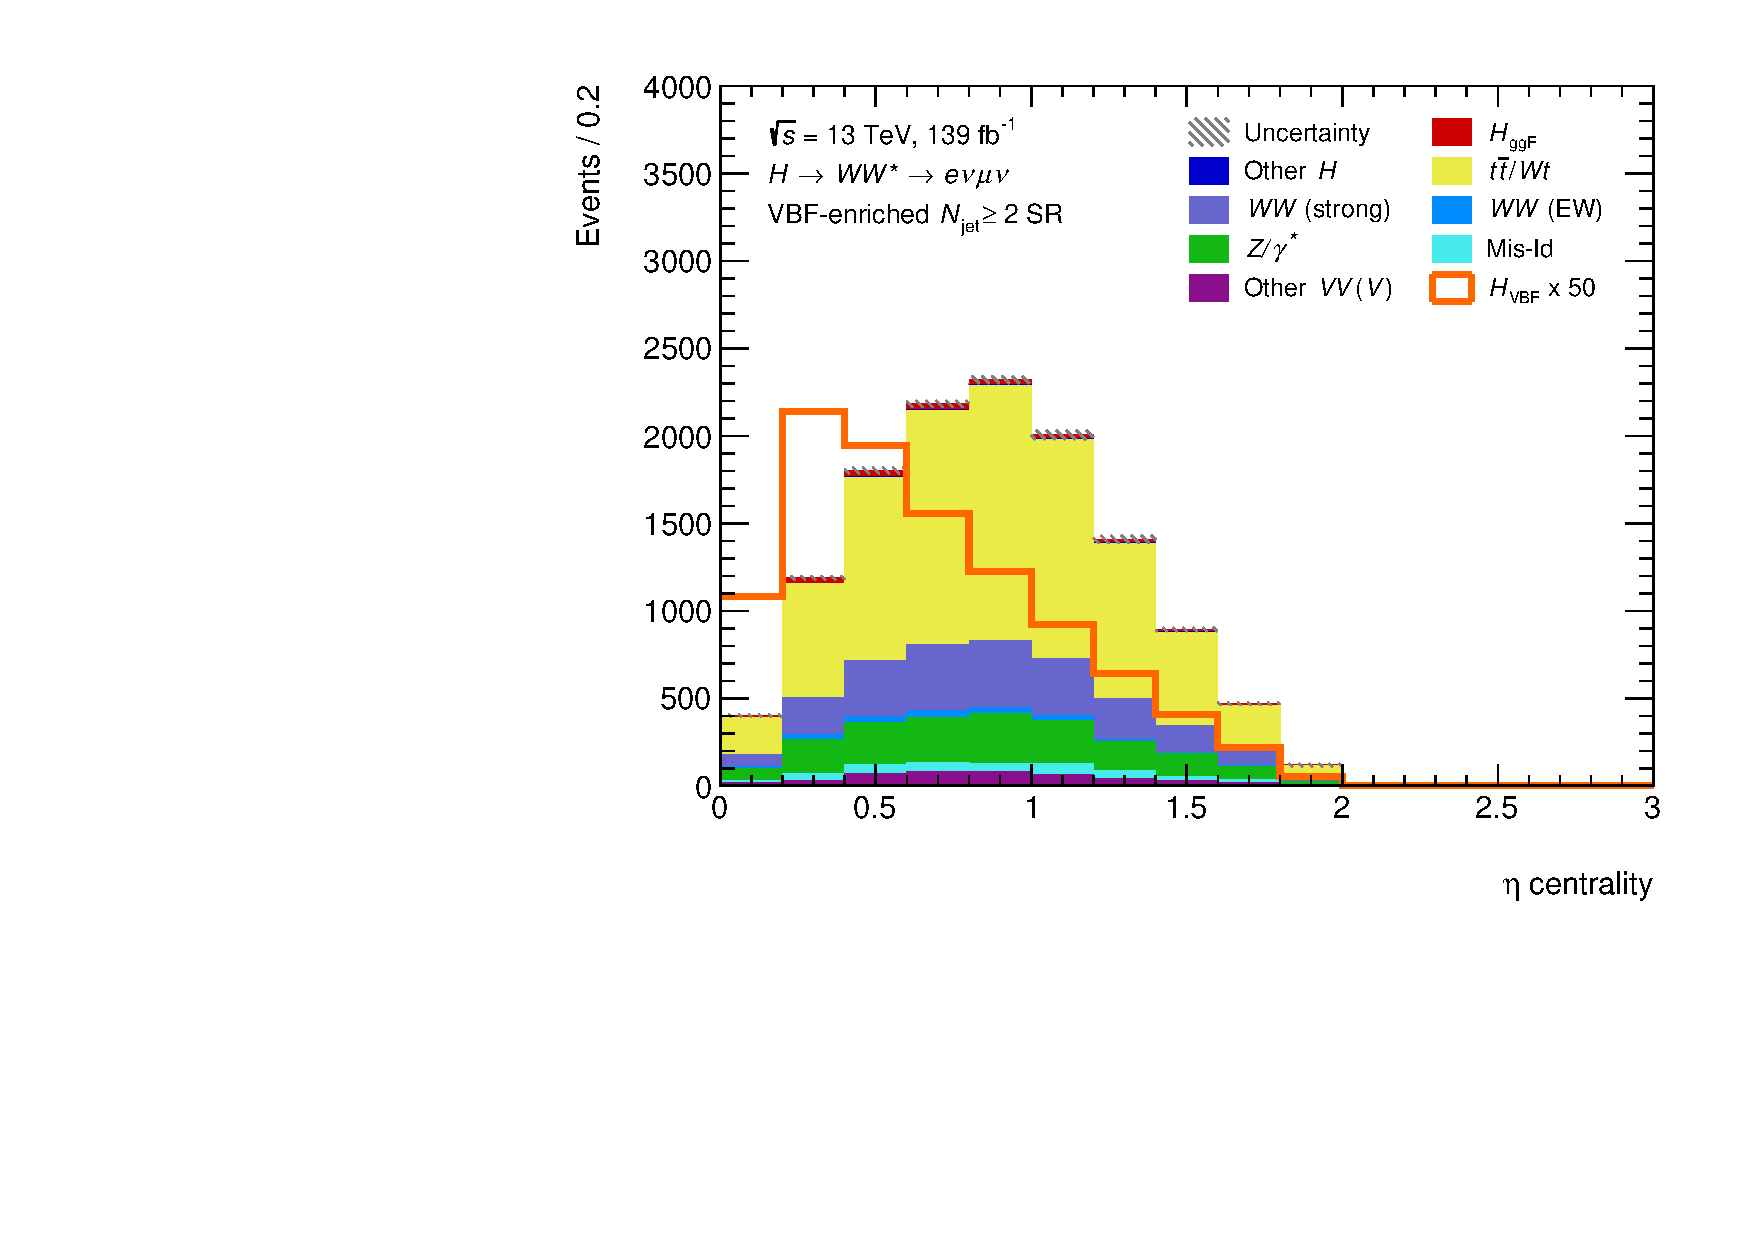
\includegraphics[width=0.32\textwidth]{figures/hww/dnn/blinded/run2-emme-CutVBF_SR-contOLV-lin.pdf} \hfill
        \label{fig:dnn-inputs-post-fit-3}
    } \\
    \subfloat[$\mlonejtwo$]{
        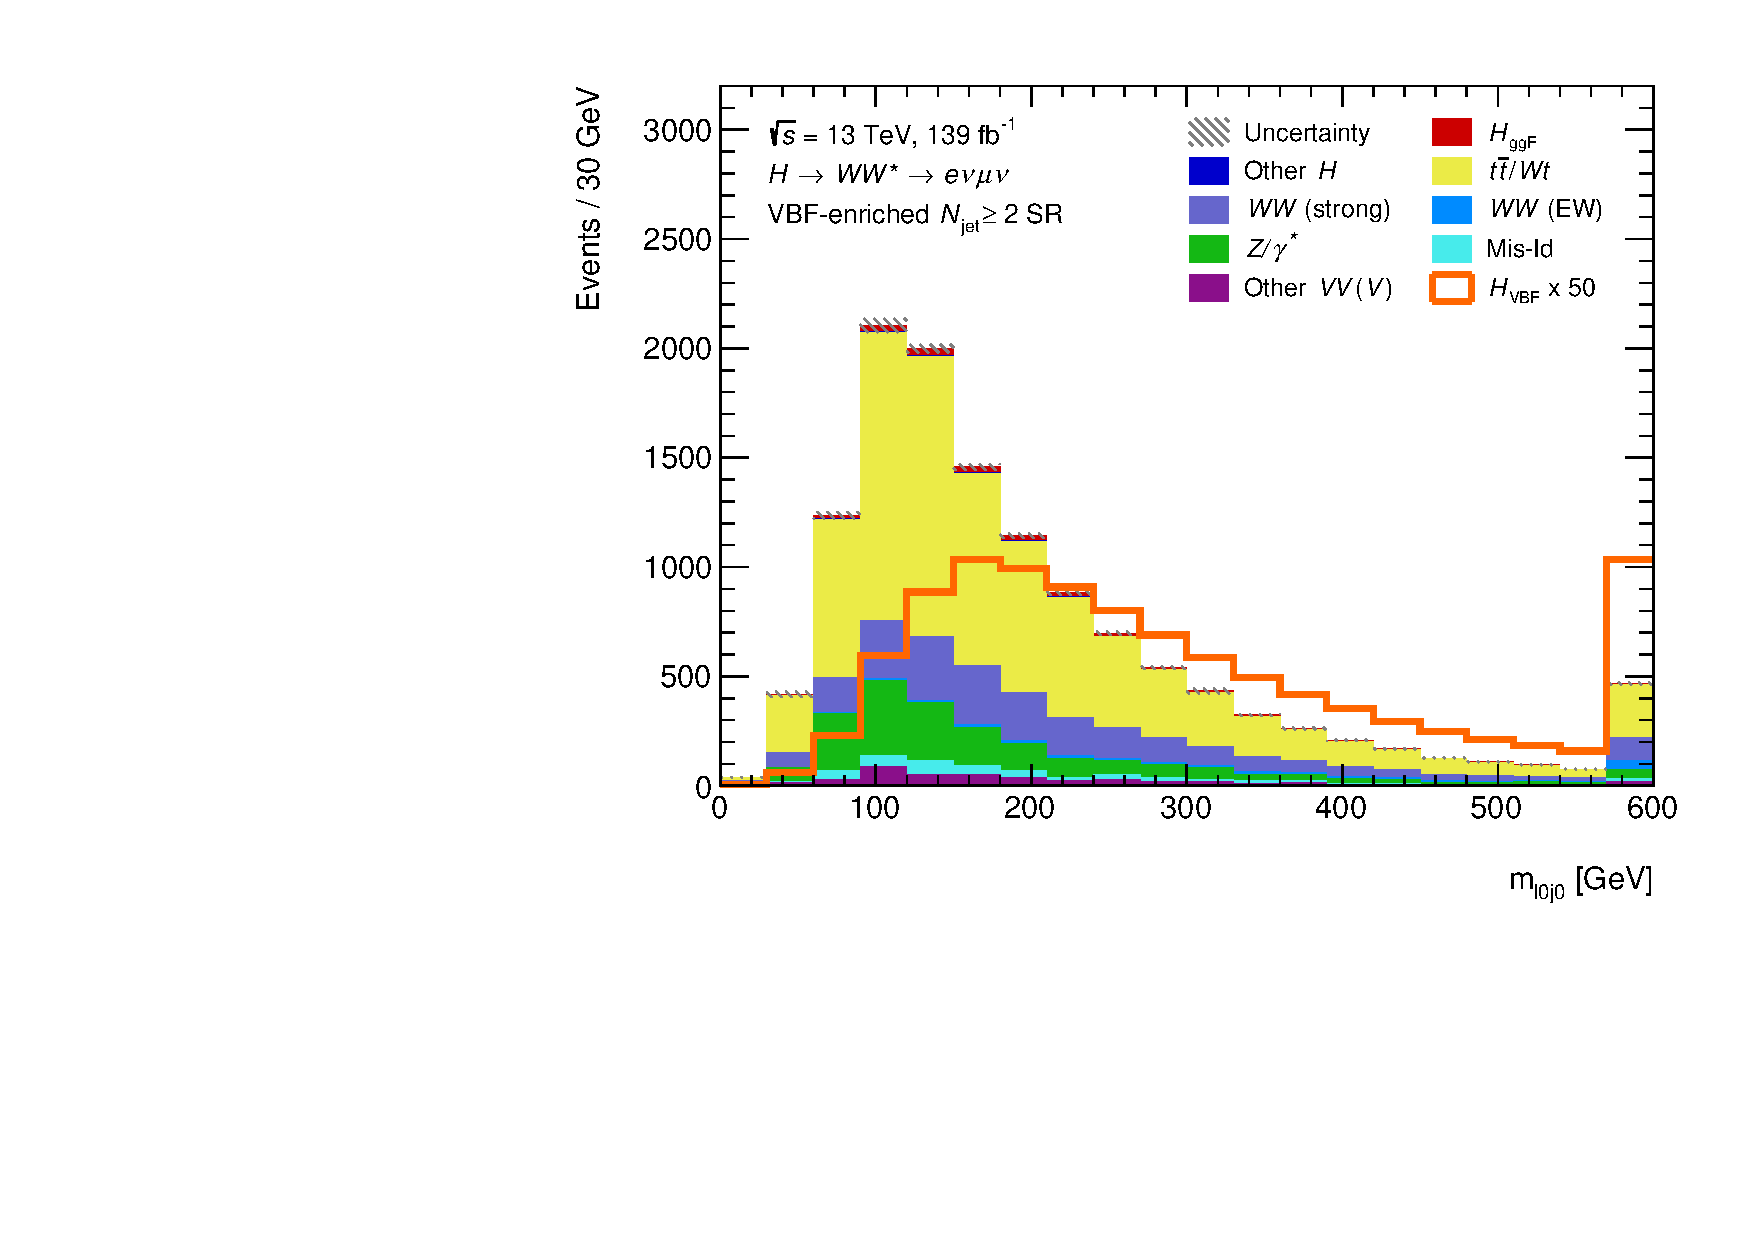
\includegraphics[width=0.32\textwidth]{figures/hww/dnn/blinded/run2-emme-CutVBF_SR-Ml0j0-lin.pdf} \hfill
        \label{fig:dnn-inputs-post-fit-4}
    }
    \subfloat[$\mltwojone$]{
        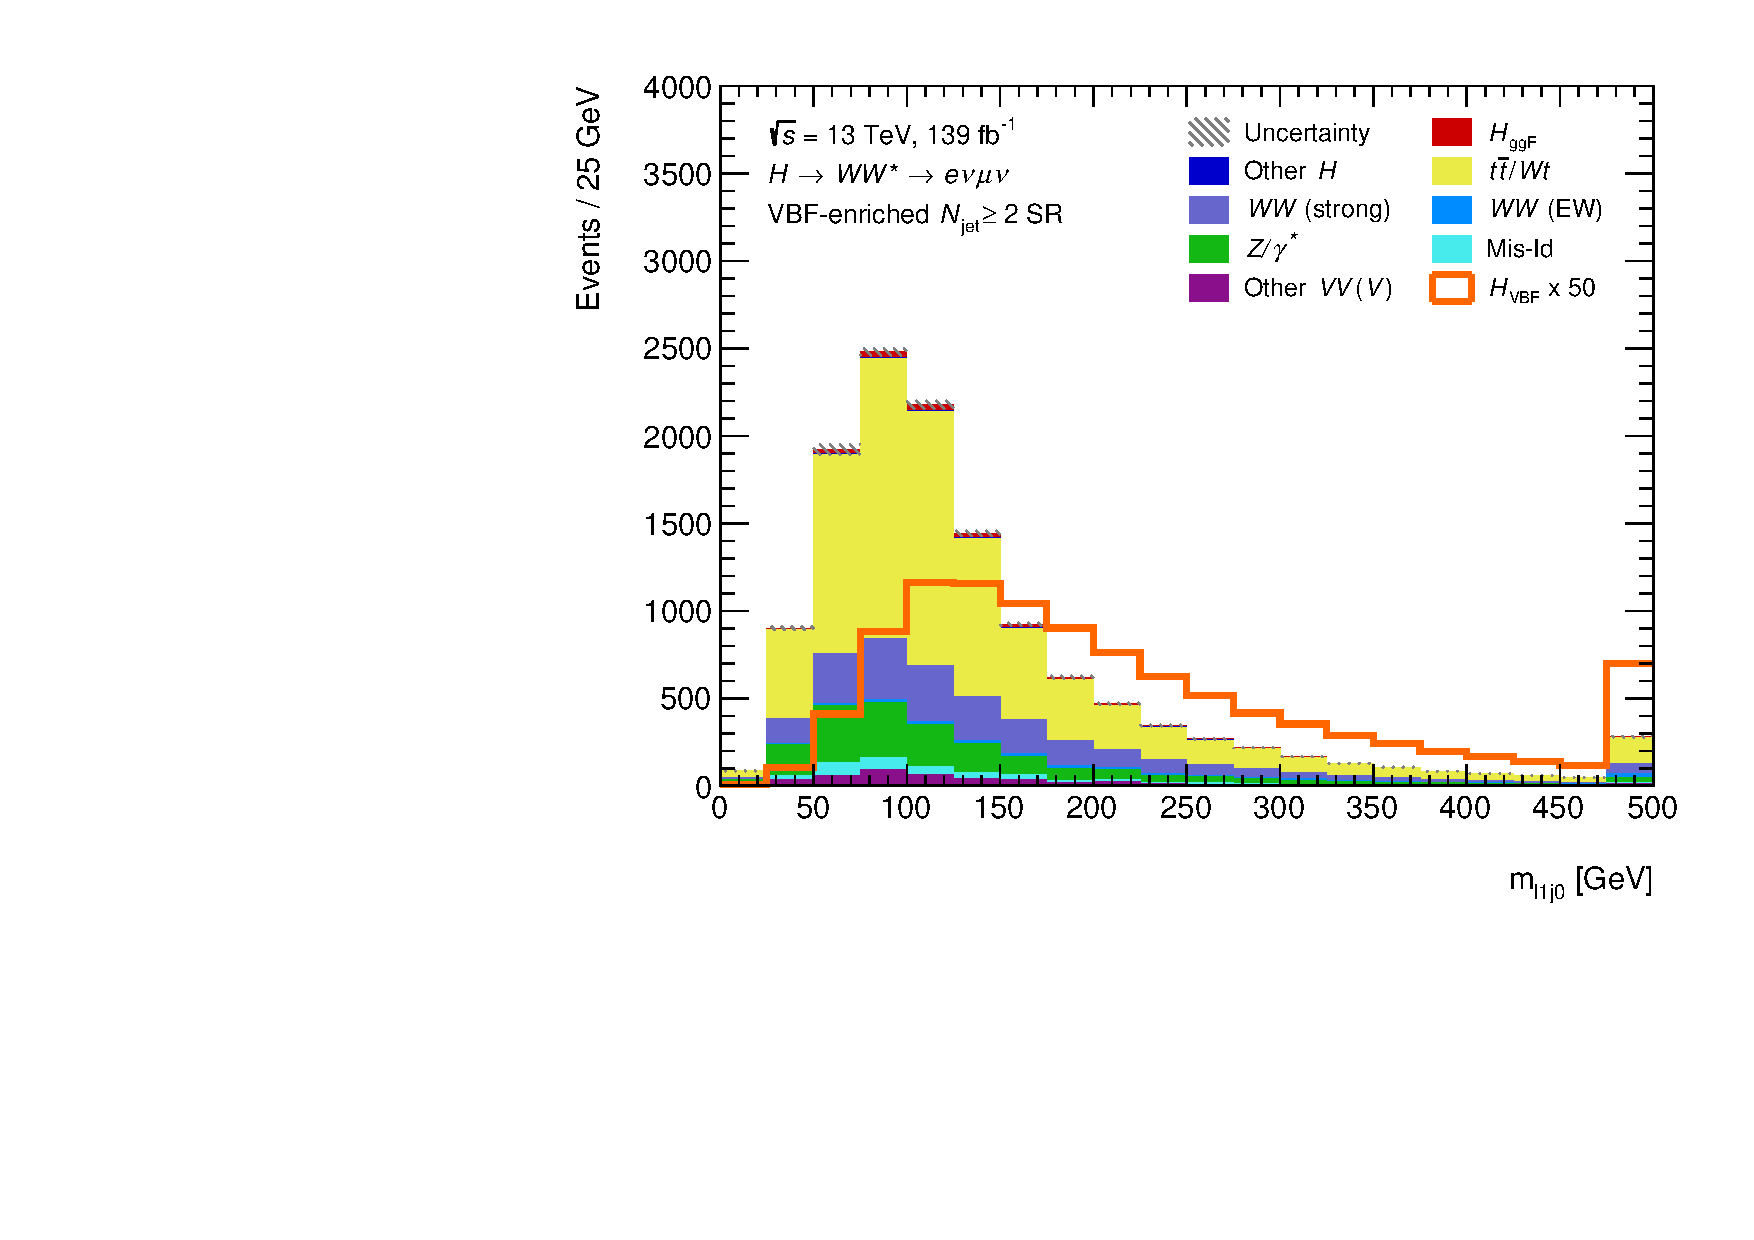
\includegraphics[width=0.32\textwidth]{figures/hww/dnn/blinded/run2-emme-CutVBF_SR-Ml1j0-lin.pdf} \hfill
        \label{fig:dnn-inputs-post-fit-5}
    }
    \subfloat[$\mlonejtwo$]{
        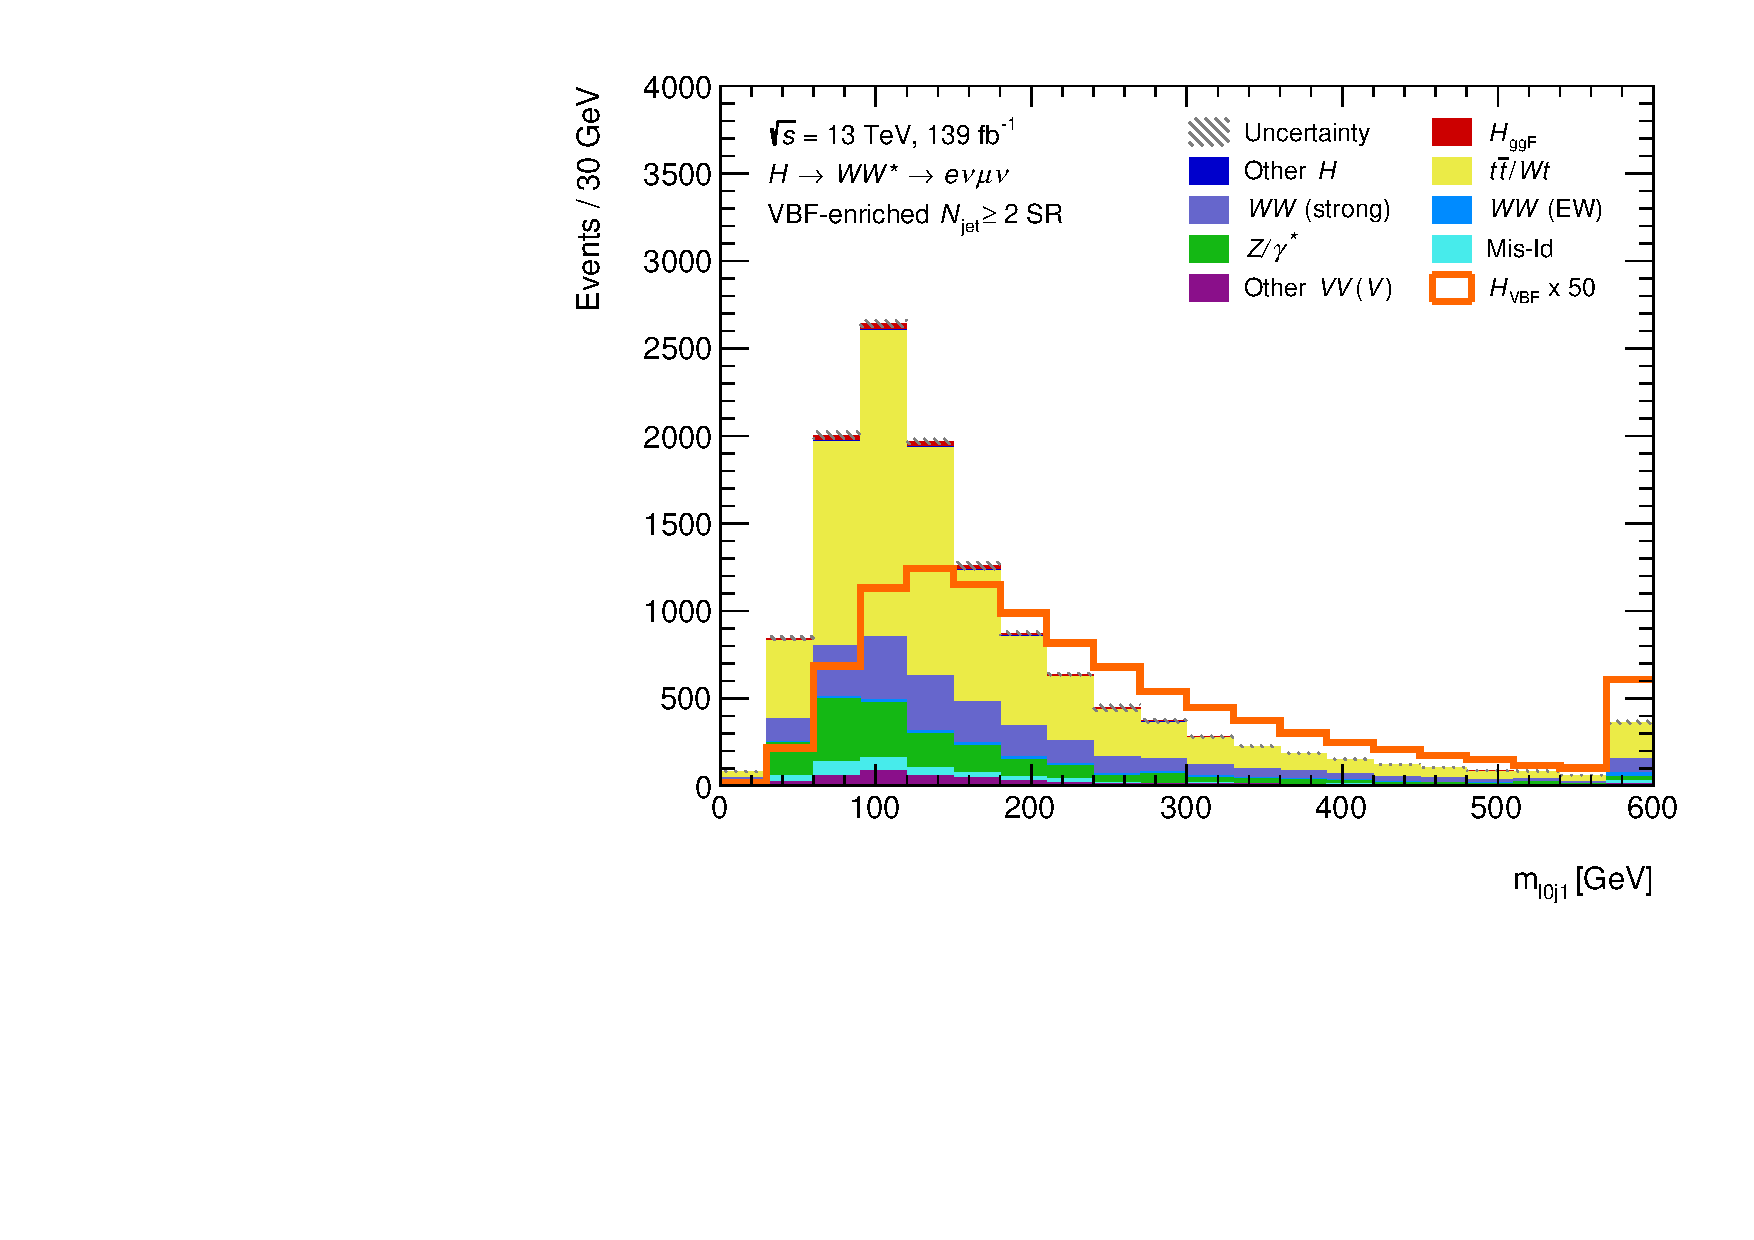
\includegraphics[width=0.32\textwidth]{figures/hww/dnn/blinded/run2-emme-CutVBF_SR-Ml0j1-lin.pdf} \hfill
        \label{fig:dnn-inputs-post-fit-6}
    } \\
    \subfloat[$\mltwojtwo$]{
        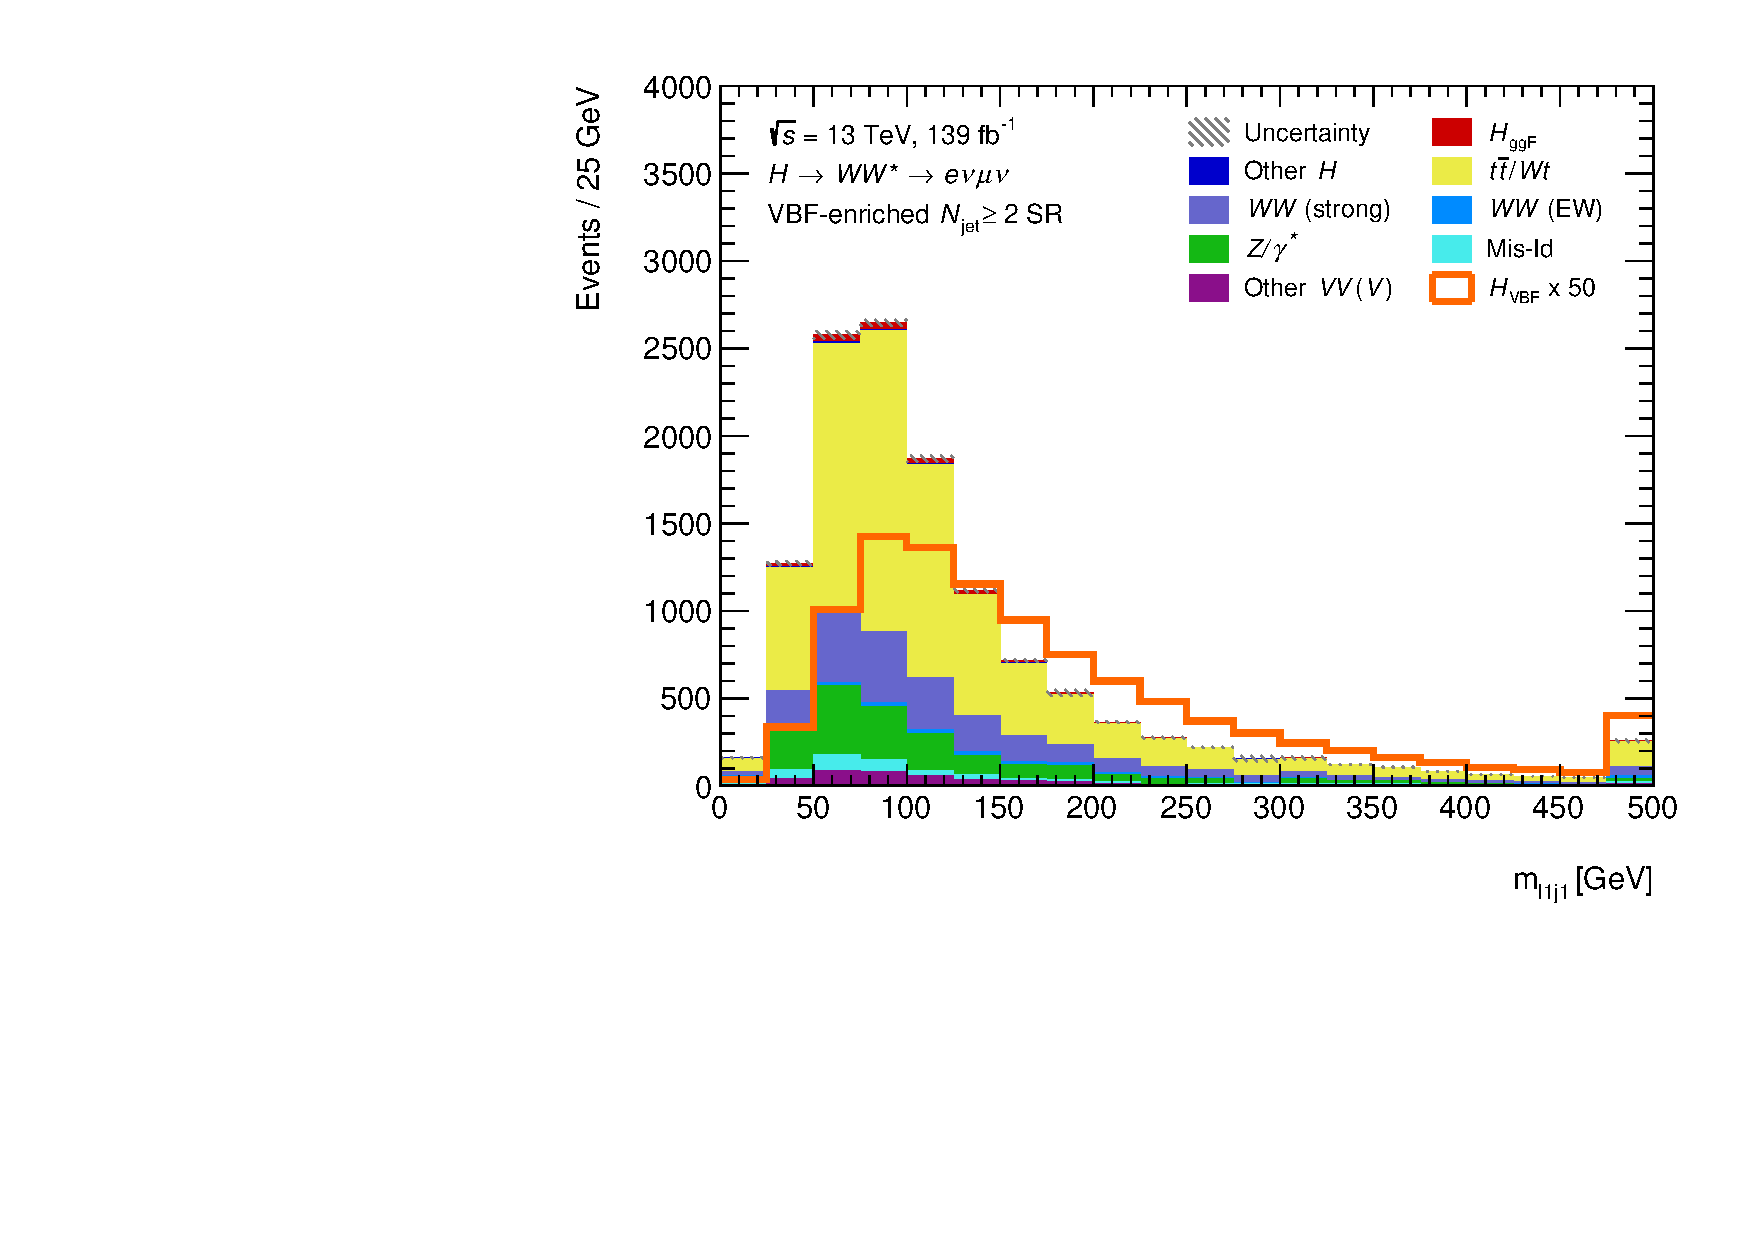
\includegraphics[width=0.32\textwidth]{figures/hww/dnn/blinded/run2-emme-CutVBF_SR-Ml1j1-lin.pdf} \hfill
        \label{fig:dnn-inputs-post-fit-7}
    }
    \subfloat[$\pTjone$]{
        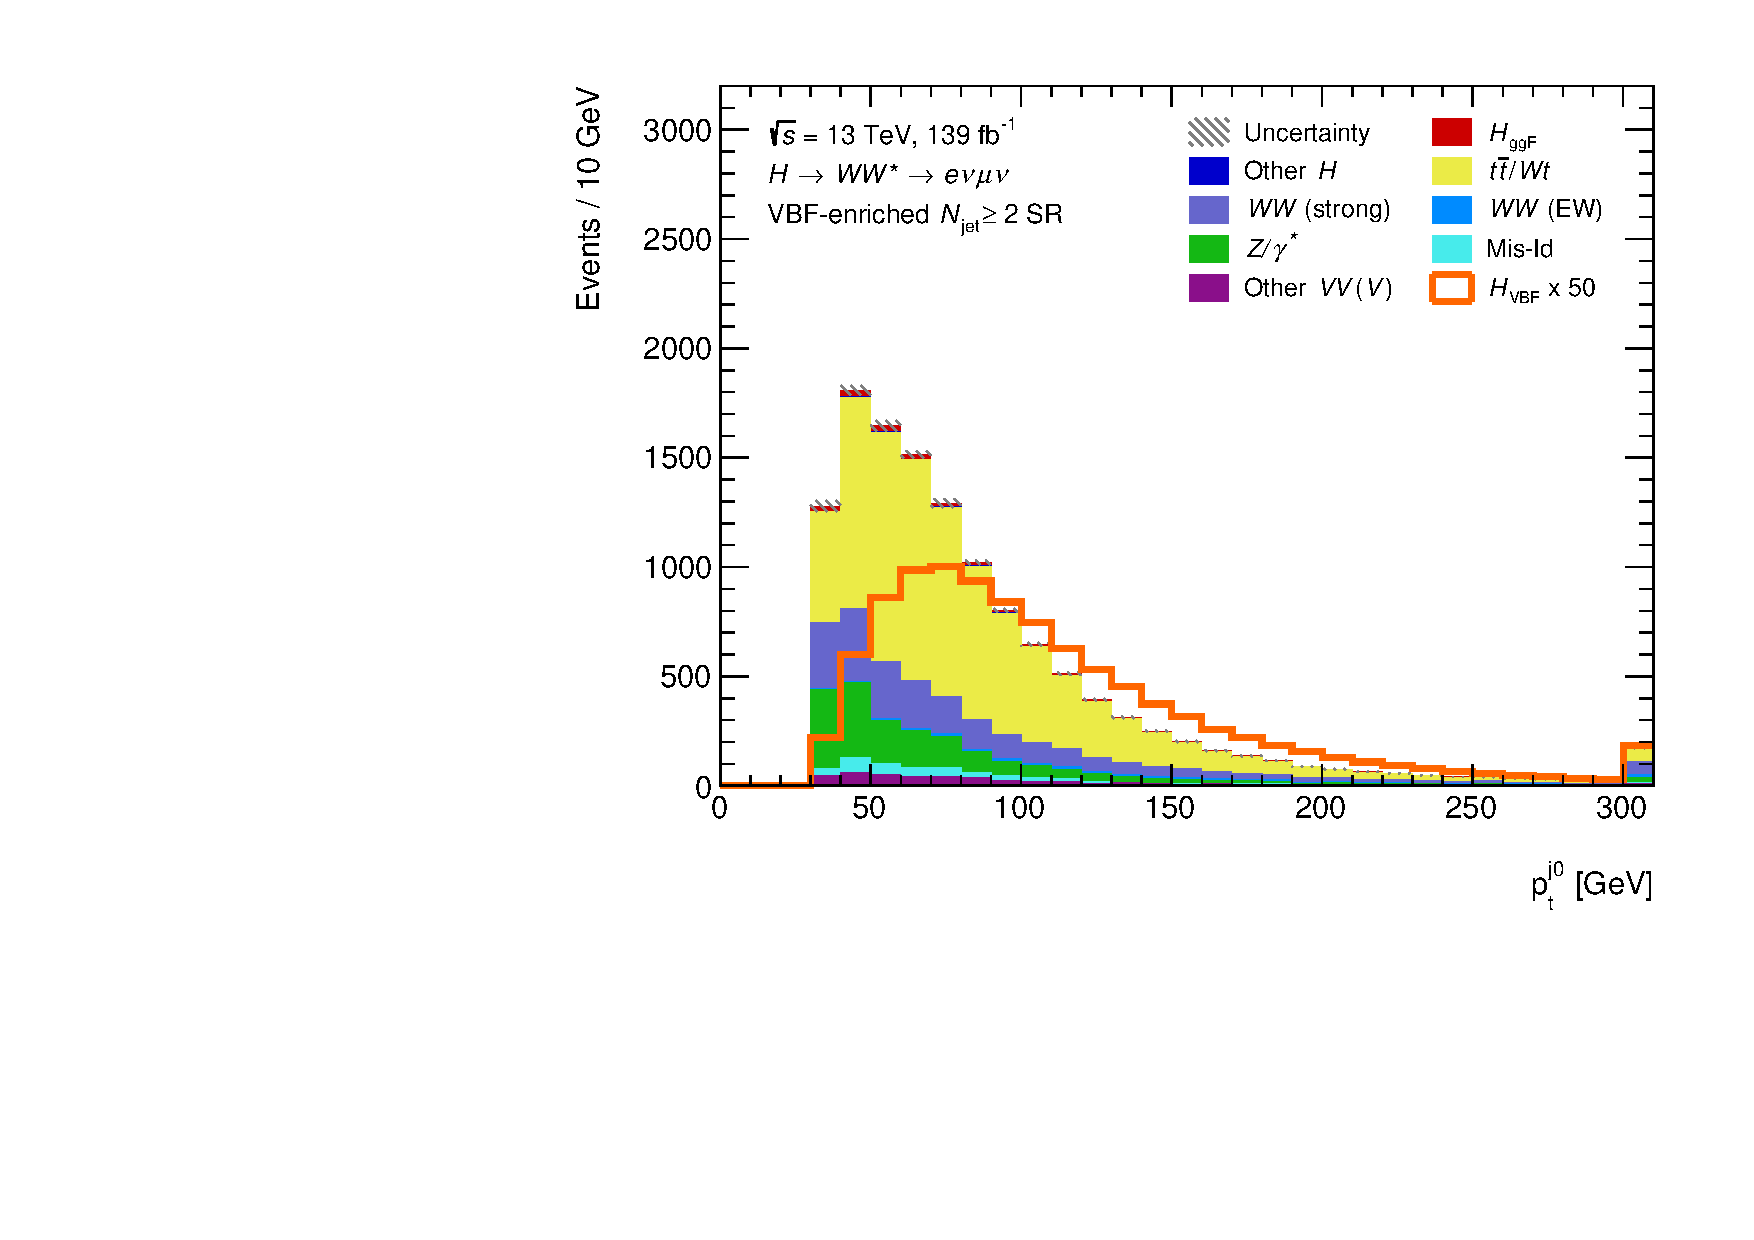
\includegraphics[width=0.32\textwidth]{figures/hww/dnn/blinded/run2-emme-CutVBF_SR-leadJetPt-lin.pdf} \hfill
        \label{fig:dnn-inputs-post-fit-8}
    }
    \subfloat[$\pTjtwo$]{
        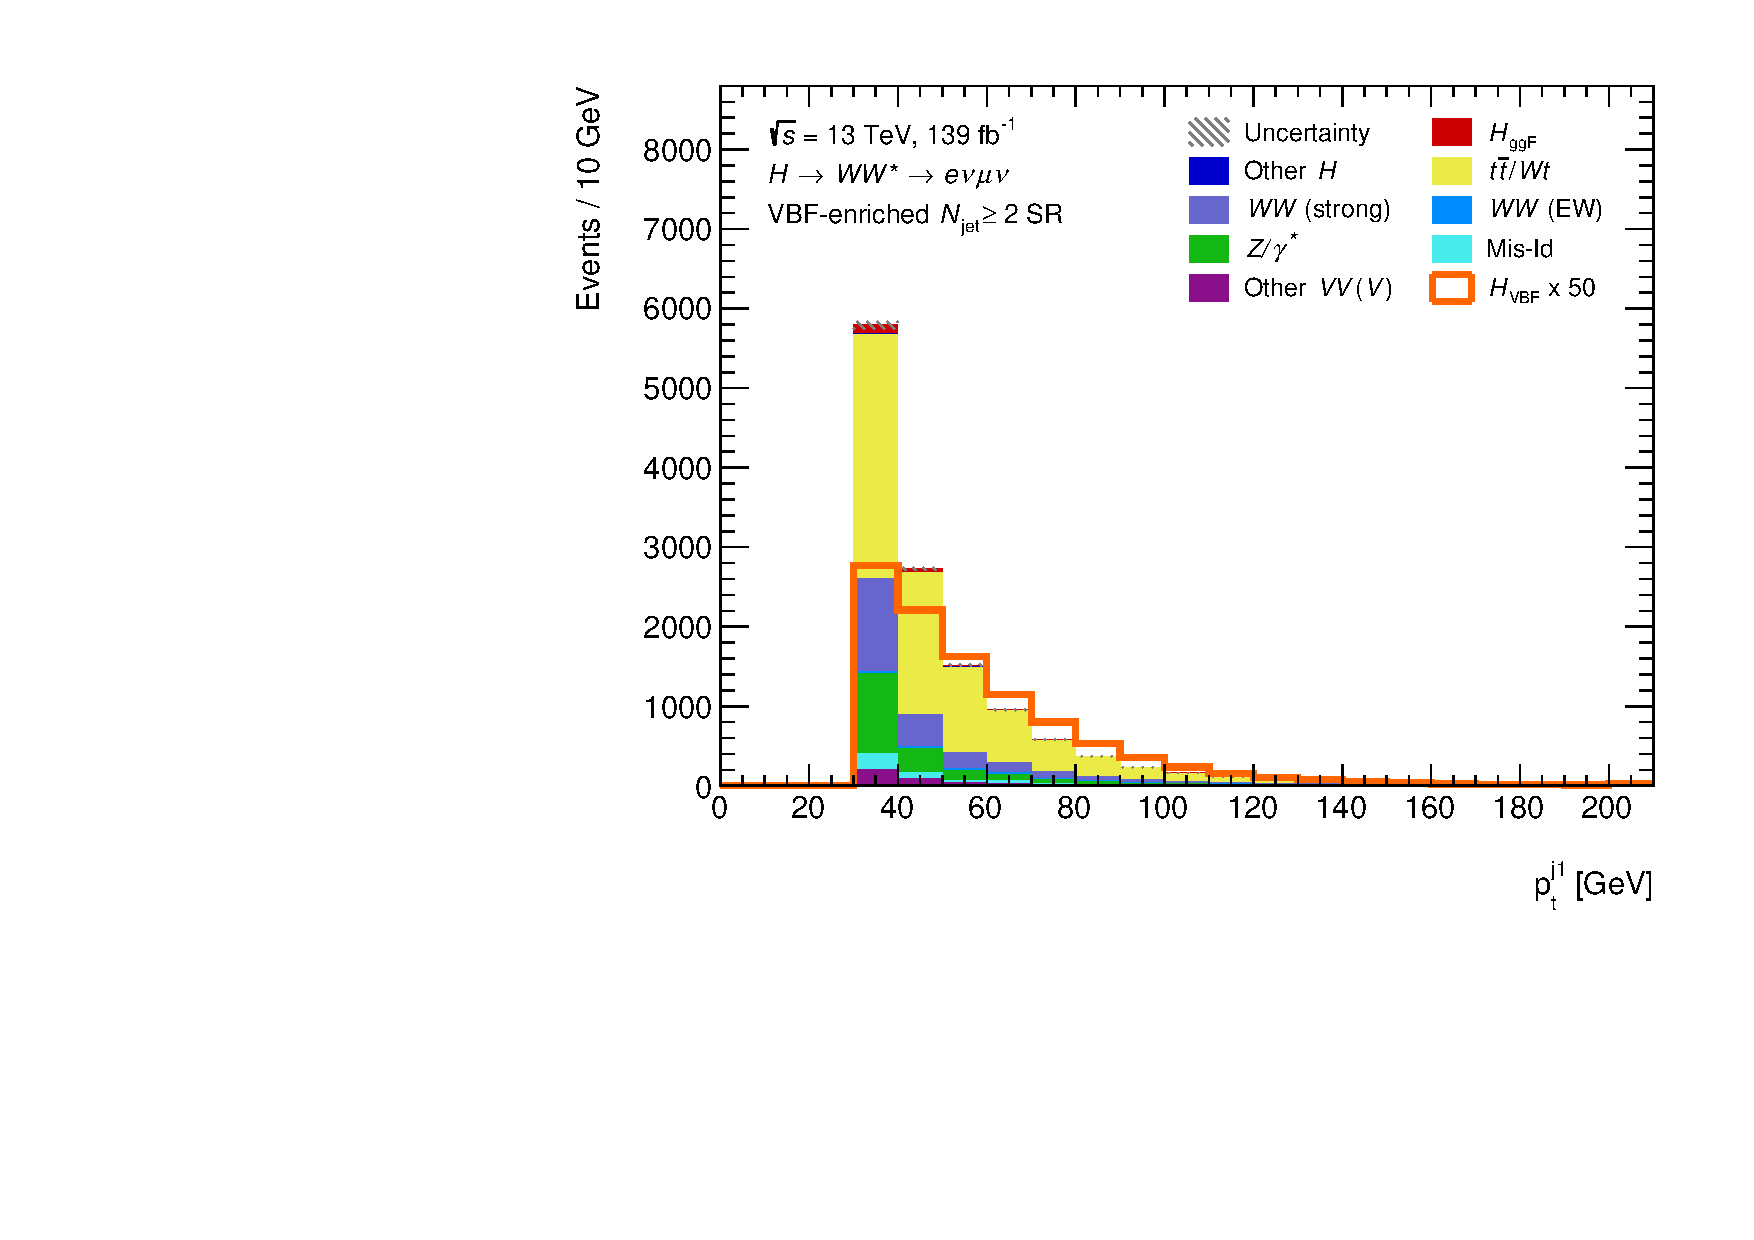
\includegraphics[width=0.32\textwidth]{figures/hww/dnn/blinded/run2-emme-CutVBF_SR-subleadJetPt-lin.pdf} \hfill
        \label{fig:dnn-inputs-post-fit-9}
    } \\
    \subfloat[$\pTjthree$]{
        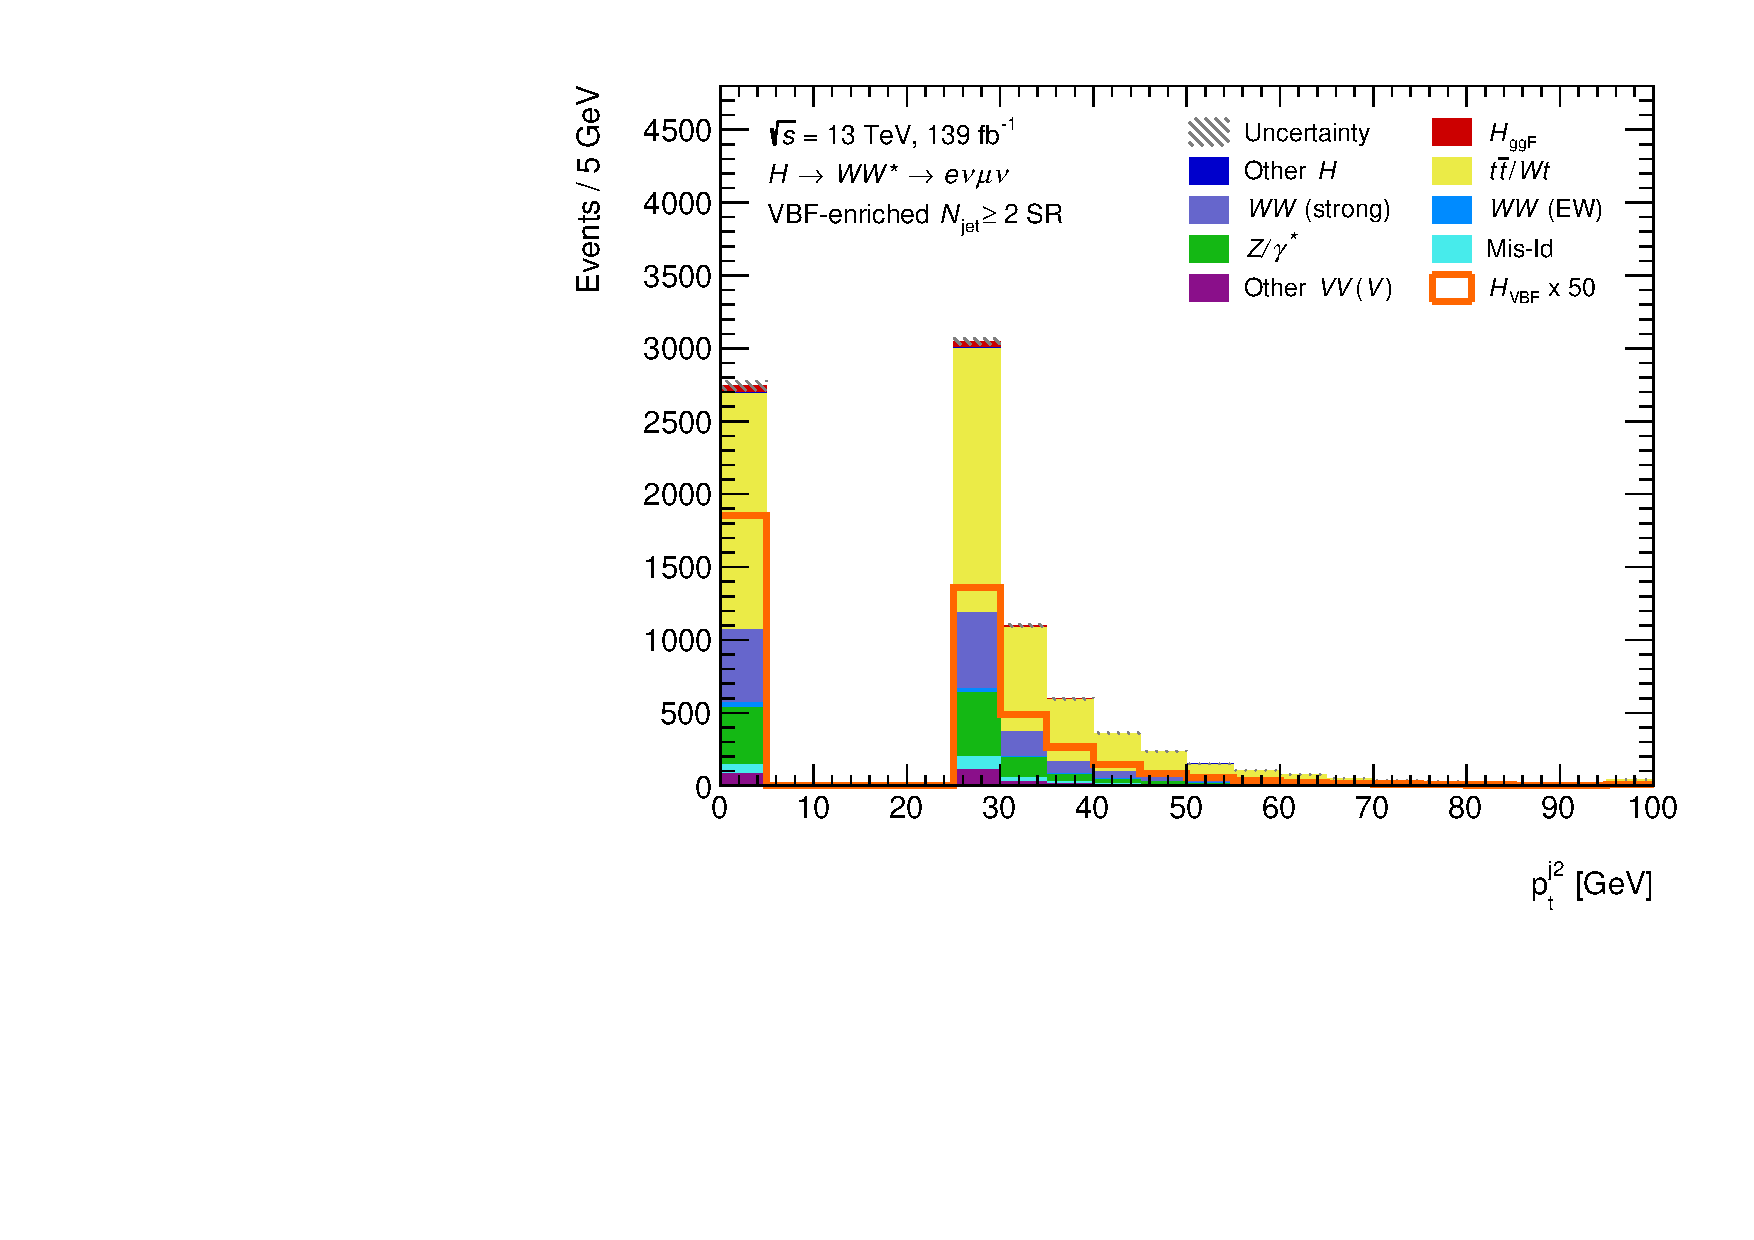
\includegraphics[width=0.32\textwidth]{figures/hww/dnn/blinded/run2-emme-CutVBF_SR-thirdJetPt-lin.pdf} \hfill
        \label{fig:dnn-inputs-post-fit-10}
    }
    {\caption{Distributions of 10 of the 15 DNN input variables targeting the VBF topology. The distributions are shown in the VBF SR for simulated samples only. The solid orange line shows the expected VBF signal scaled by a factor of 50. The last bin of the distributions include the overflow.
            \label{fig:dnn-inputs-post-fit1} }}
\end{figure}

\paragraph{\HWW decay}
The distinct features of the \HWW decay (see \cref{subsec:signal-bkg-characterisation}) are exploited with the \dphill, \mll, and \mT variables.
The separation between the VBF signal and the backgrounds is clearly visible (see \cref{fig:dnn-inputs-post-fit2-1,fig:dnn-inputs-post-fit2-2,fig:dnn-inputs-post-fit2-3}).

\paragraph{Top-background suppression}
Two additional observables are used that take into account information about the entire event:
The total transverse momentum, \pttot, defined as the magnitude of the vectorial sum of the \pT of all selected objects\footnote{Specifically, $\pttot = | \vpTlone + \vpTltwo + \vmet + \sum_{i \in \text{jets}} \vpTjetsi |$}, helps discriminating events with significant soft-gluon radiation for example in \ttbar events; and the \METSig provides discrimination between events with real undetected high-\pT particles, such as neutrinos, and events where the \MET is the result of resolution effects. Both observables take on average smaller values for the VBF signal than the sum of backgrounds (see \cref{fig:dnn-inputs-post-fit2-4,fig:dnn-inputs-post-fit2-5}).

% \begin{figure}[h]
%     \centering
%     {\caption{Distributions of $\mlonejone$, $\mltwojone$, $\mlonejtwo$, and $\mltwojtwo$ in the VBF signal region.
%             Each row shows one variable with different cuts on the DNN output distribution being applied in different columns.
%             \label{fig:dnn-inputs-vbf-top2} }}
% \end{figure}
\begin{figure}[ht]
    \centering
    \subfloat[$\dphill$]{
        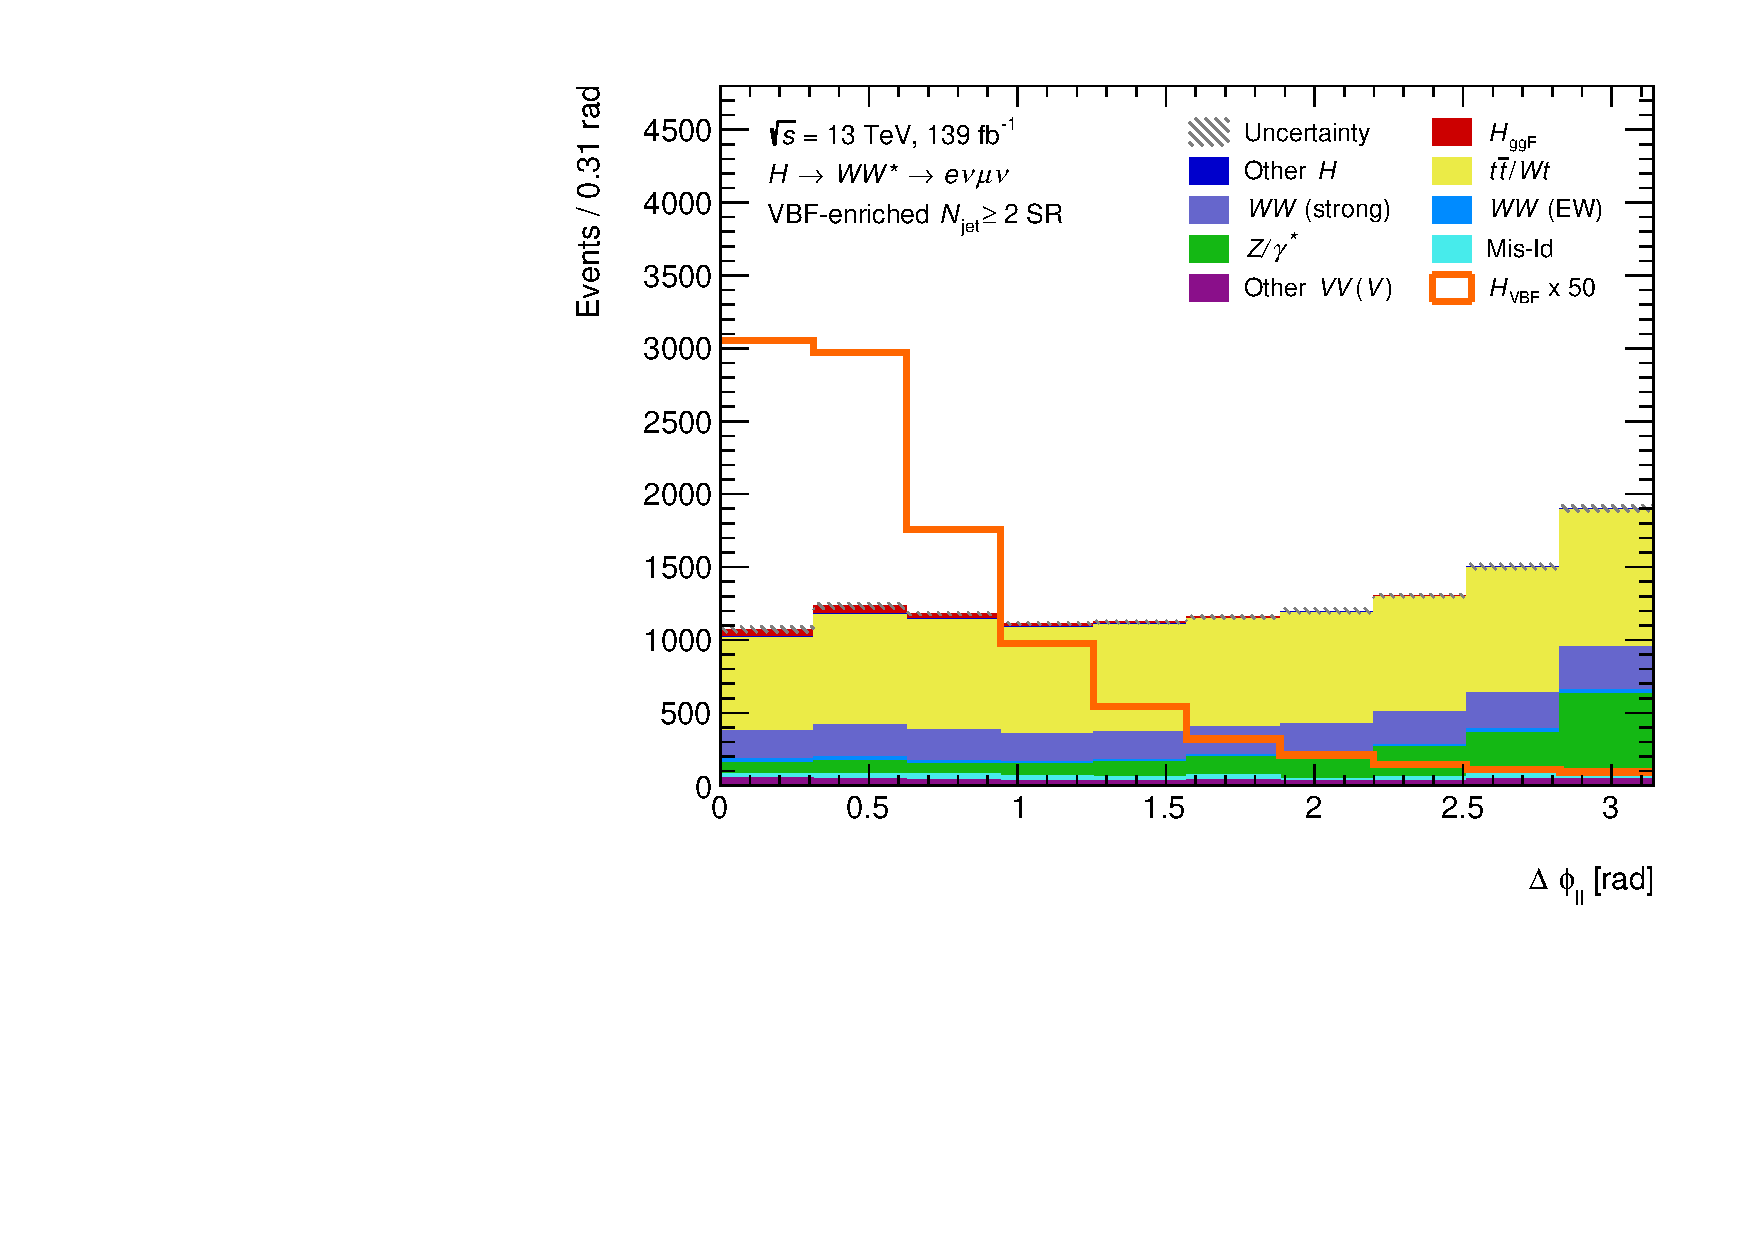
\includegraphics[width=0.32\textwidth]{figures/hww/dnn/blinded/run2-emme-CutVBF_SR-DPhill-lin.pdf} \hfill
        \label{fig:dnn-inputs-post-fit2-1}
    }
    \subfloat[$\mll$]{
        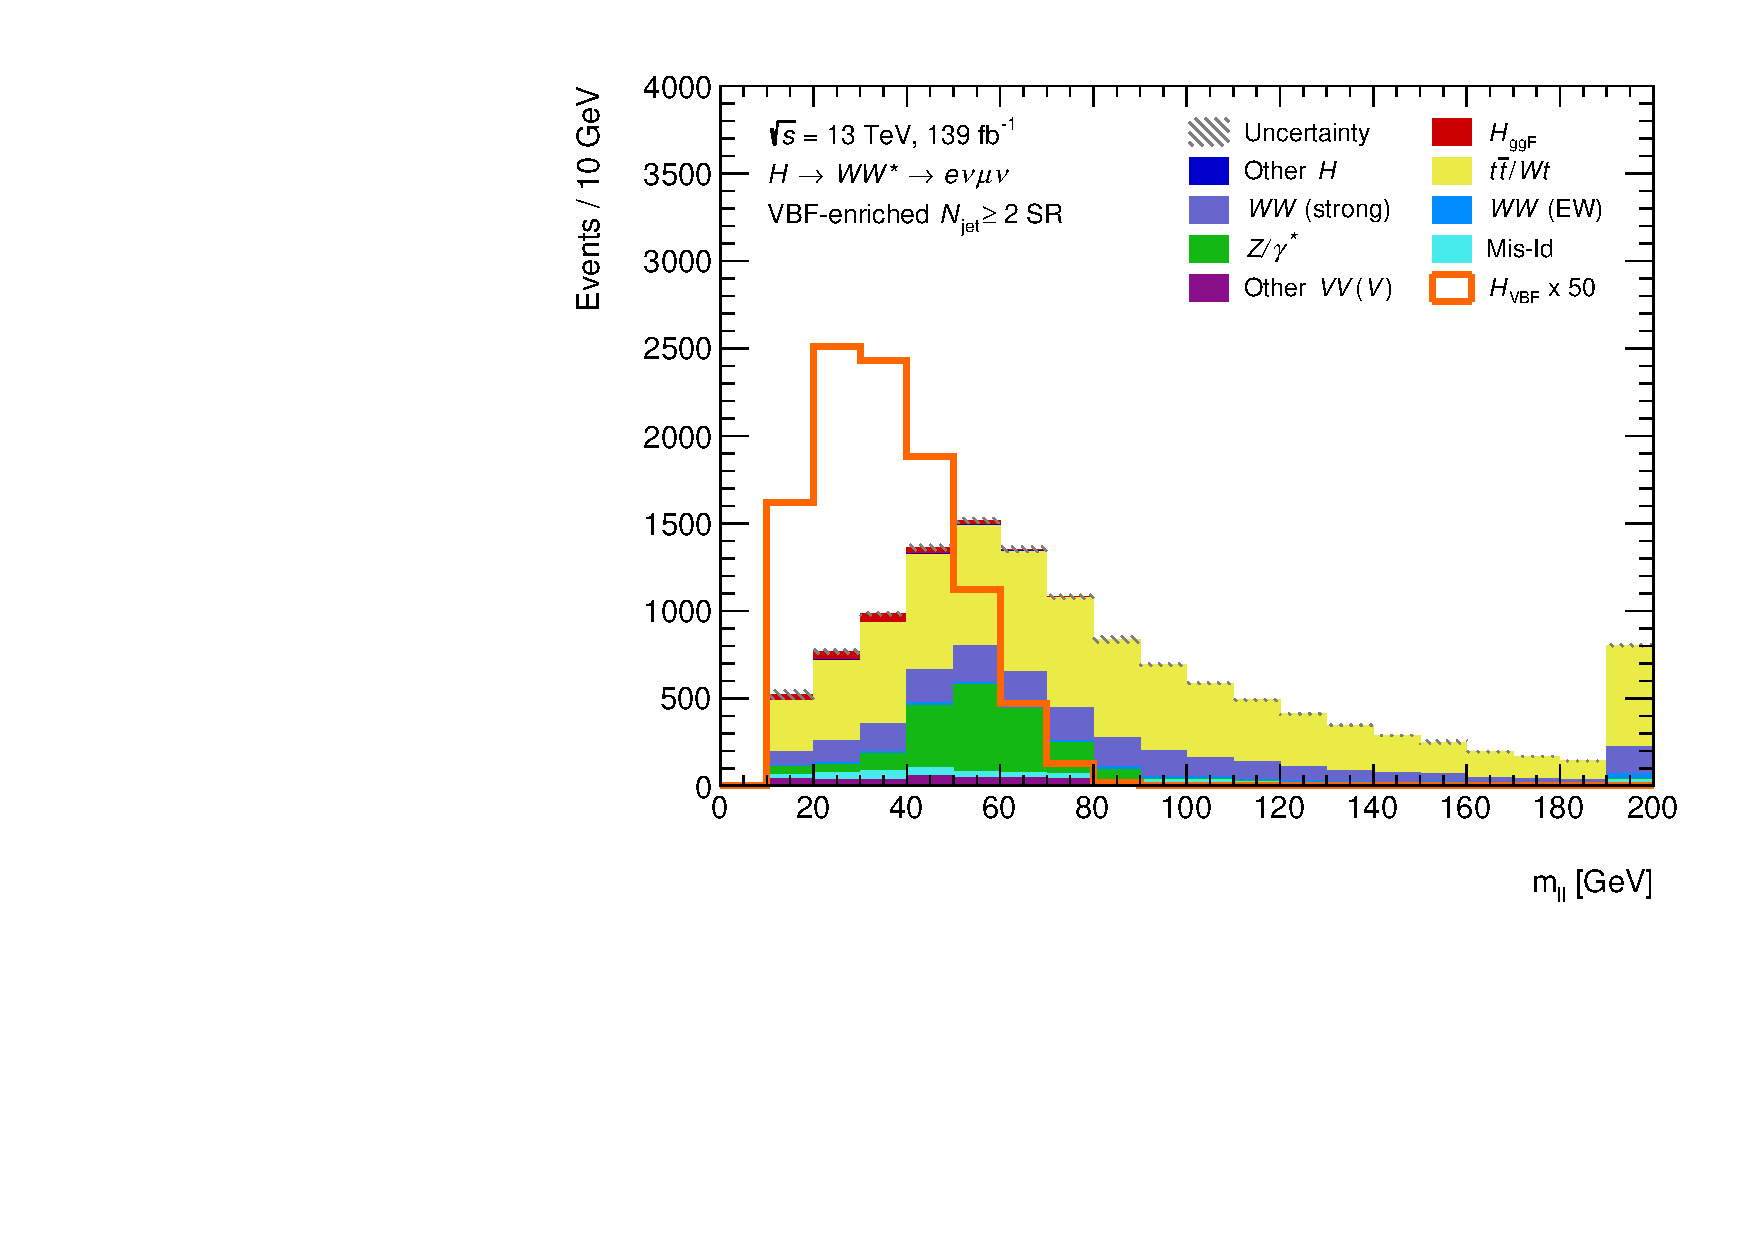
\includegraphics[width=0.32\textwidth]{figures/hww/dnn/blinded/run2-emme-CutVBF_SR-Mll-lin.pdf}
        \label{fig:dnn-inputs-post-fit2-2}
    }
    \subfloat[$\mT$]{
        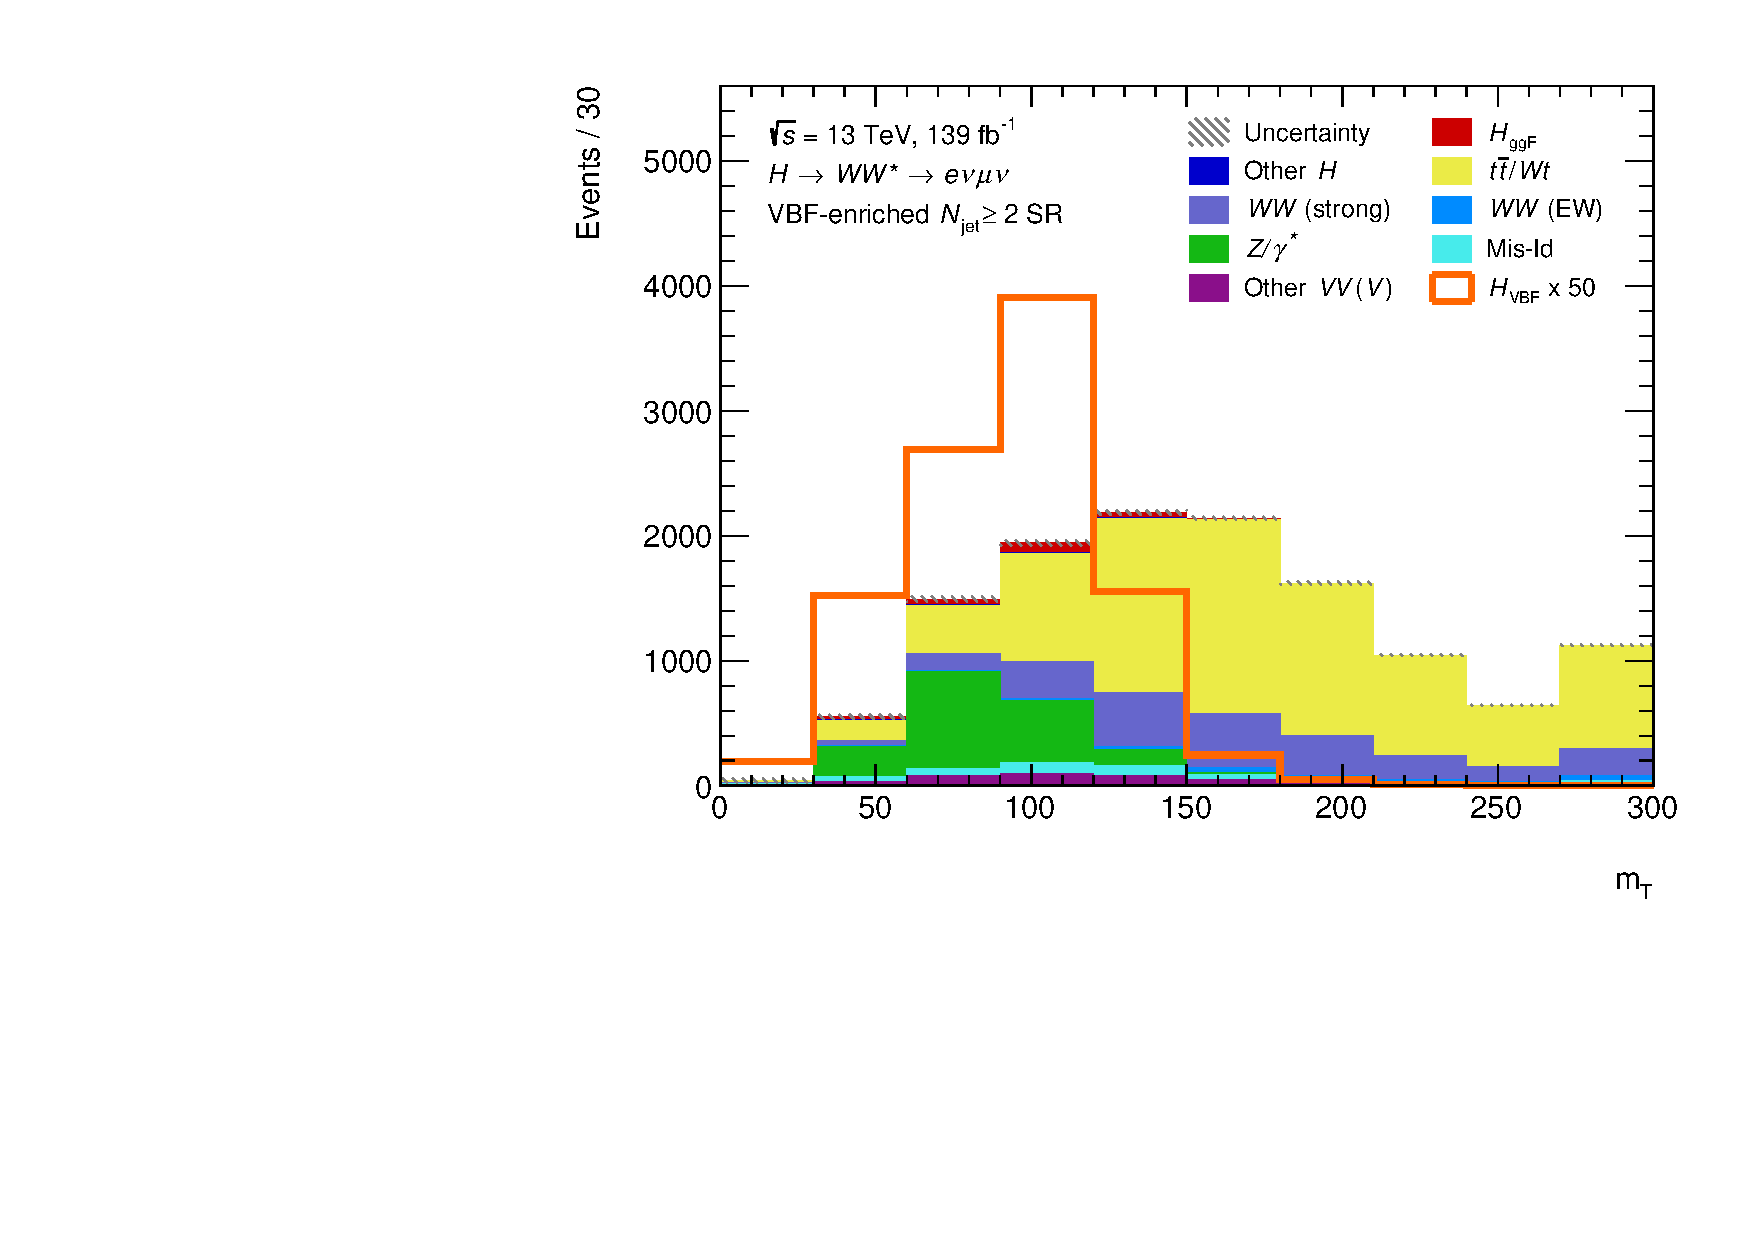
\includegraphics[width=0.32\textwidth]{figures/hww/dnn/blinded/run2-emme-CutVBF_SR-MT-lin.pdf} \hfill
        \label{fig:dnn-inputs-post-fit2-3}
    } \\
    \subfloat[$\pttot$]{
        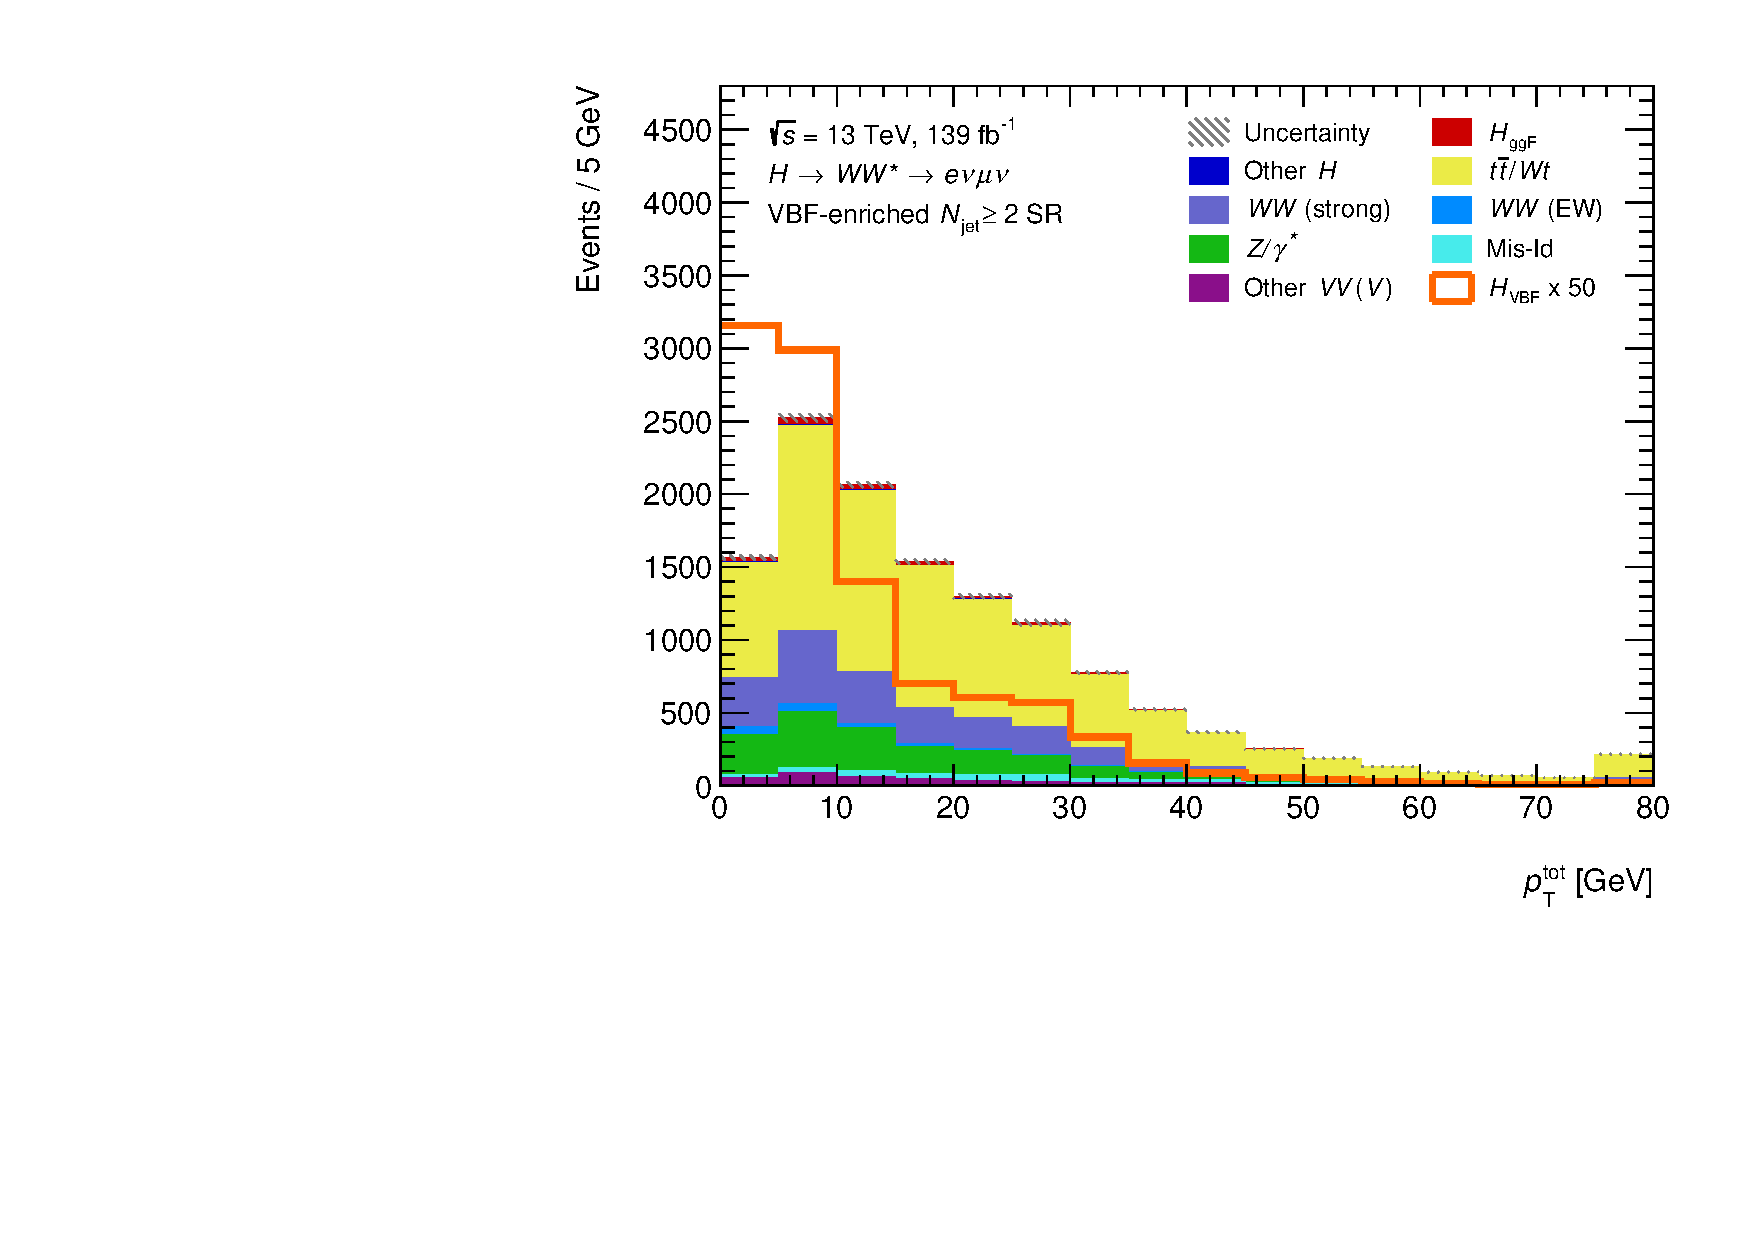
\includegraphics[width=0.32\textwidth]{figures/hww/dnn/blinded/run2-emme-CutVBF_SR-PtTot-lin.pdf} \hfill
        \label{fig:dnn-inputs-post-fit2-4}
    }
    \subfloat[$\METSig$]{
        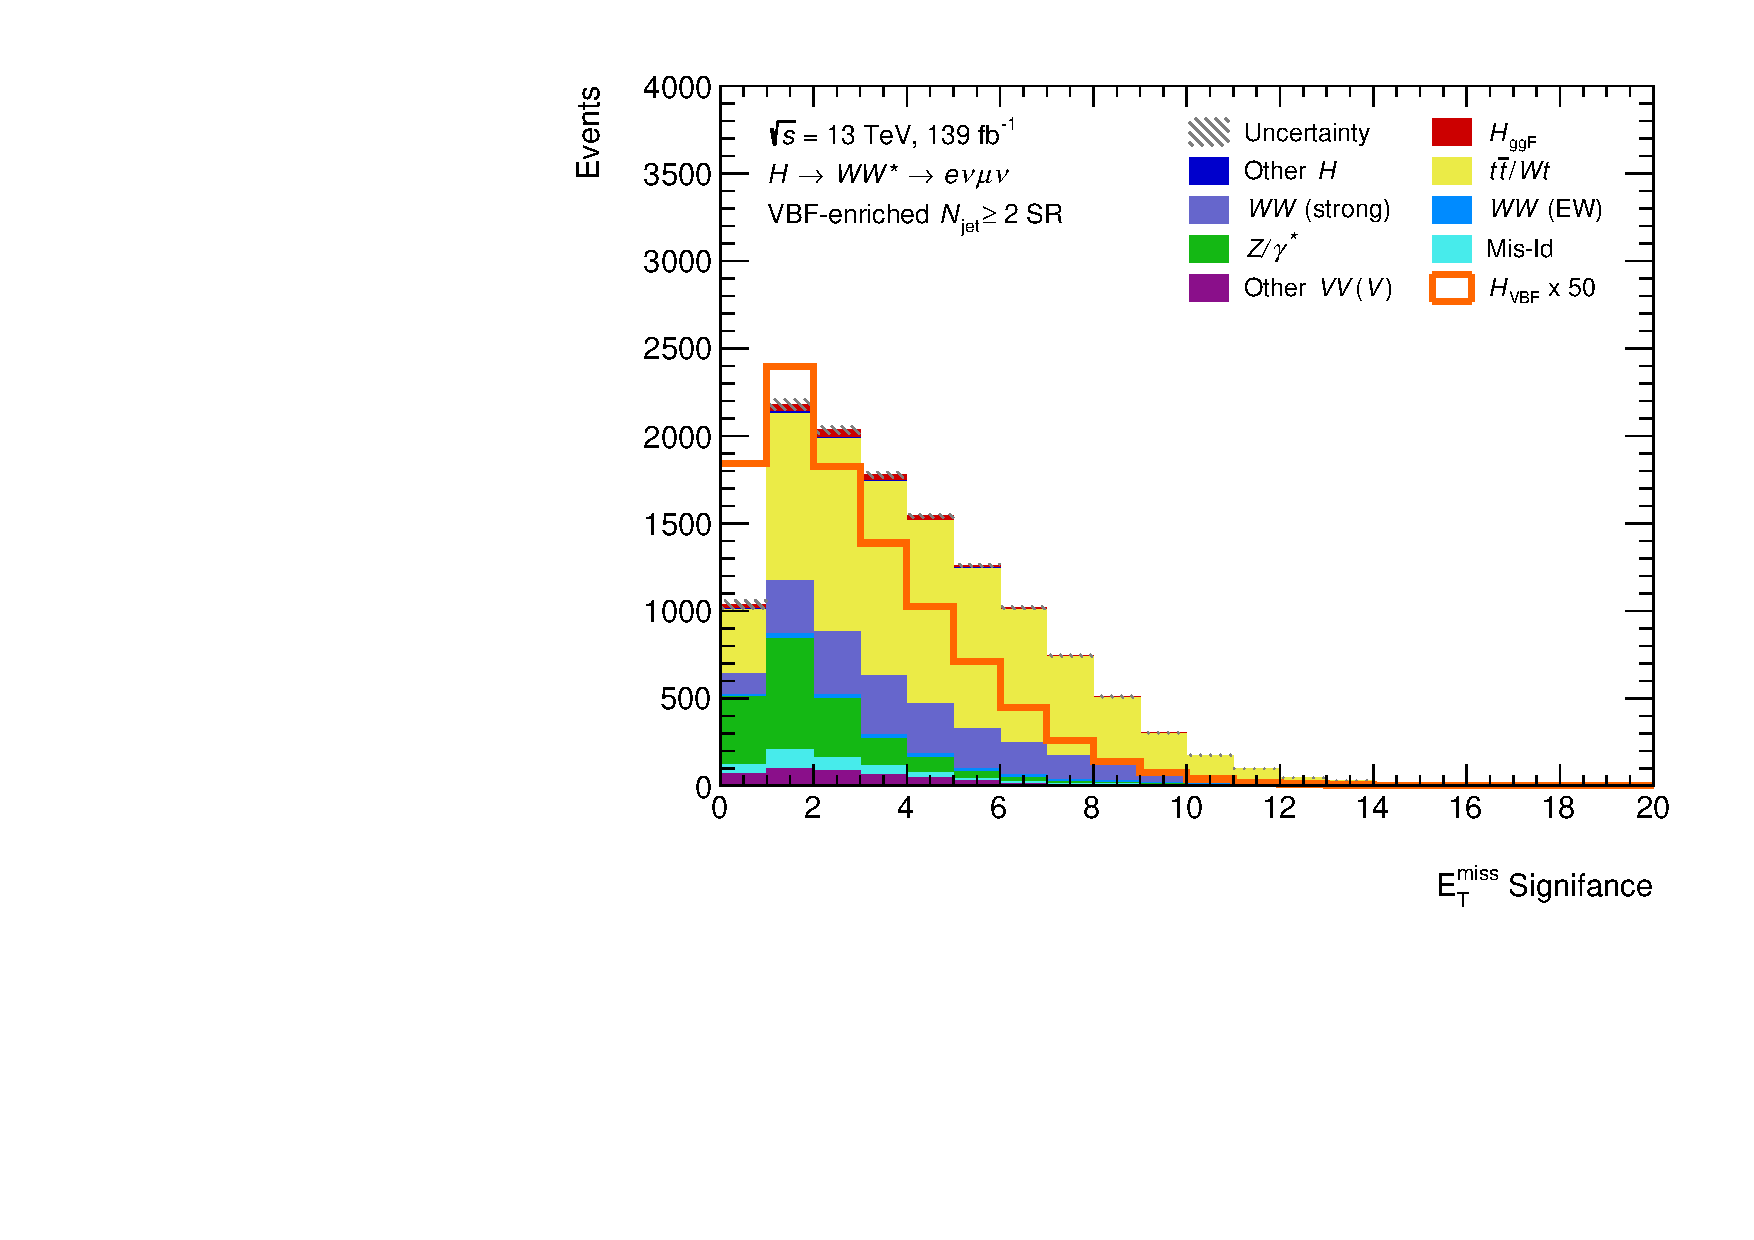
\includegraphics[width=0.32\textwidth]{figures/hww/dnn/blinded/run2-emme-CutVBF_SR-METSig_broad-lin.pdf} \hfill
        \label{fig:dnn-inputs-post-fit2-5}
    }
    {\caption{
            Distributions of 5 of the 15 DNN input variables targeting the \HWW decay and top-quark suppression. The distributions are shown in the VBF SR for simulated samples only. The solid orange line shows the expected VBF signal scaled by a factor of 50. The last bin of the distributions include the overflow.
            \label{fig:dnn-inputs-post-fit2} }}
\end{figure}
\captionsetup[subfloat]{captionskip=7pt} % space between subfloat caption and image

\paragraph{}
The material above illustrates the VBF signal discrimination in linear dimension. The major advantage of using a neural network-based approach compared to a traditional cut-based analysis is the ability to take into account multidimensional correlations between the input variables. \Cref{fig:dnn-features-correlations} indicates the correlations between the 15 input variables for the VBF signal and the non-VBF signal processes. It can be seen that the strengths of the correlations differs for several pairs of observables, in particular for the $m_{\ell_\alpha j_\beta}$ (with $\alpha, \beta = 1, 2$) and the \pTjthree observables.
% Include DNN figures (many plots!)
%\dnnfigurespostfit
\begin{figure}[ht]
    \subfloat[] {
        \newImageResizeCustom{0.48}{figures/hww/dnn/correlation-matrix-sig.pdf}
    }
    \subfloat[] {
        \newImageResizeCustom{0.48}{figures/hww/dnn/correlation-matrix-bkg.pdf}
    }
    \caption{Correlation matrix of the input features used in the VBF DNN for (a) the VBF signal and (b) the non-VBF signal processes.}
    \label{fig:dnn-features-correlations}
\end{figure}

Because the neural network is trained with simulated samples but deployed on data, it is important to validate that all input variables used are correctly modelled by the simulated samples.
Data to simulation comparison plots for representative variables are shown in \cref{sec:bkg-estimation}, specifically \cref{fig:topcr:dnn-inputs} for the top-quark CR, \cref{fig:zttcr:dnn-inputs} for the \Ztautau CR, and in \cref{fig:wwvr:dnn-inputs} for the $WW$ VR. All distributions show excellent consistency between the data and MC simulation.

The modelling of the two-dimensional correlations between the input variables is also validated.
To this end, \cref{fig:dnn-features-profiles} analyzes the two-dimensional correlations between all combinations of input variables. The compatibility between data and simulation is tested with a $\chi^2$ test.
The corresponding $p$-values determine the color of the in total 210 figures.
The slight overrepresentation of $p$-values in the ranges $0.005 < p < 0.05$ (22/210) and $p < 0.005$ (14/2010) with respect to the expectation is deemed acceptable, considering that no systematic uncertainties are included in this comparison.
%The distributions confirm that the simulated samples model the correlations in the data reasonably well.  \todo{Validate region and adapt plot}
\begin{figure}[ht]
    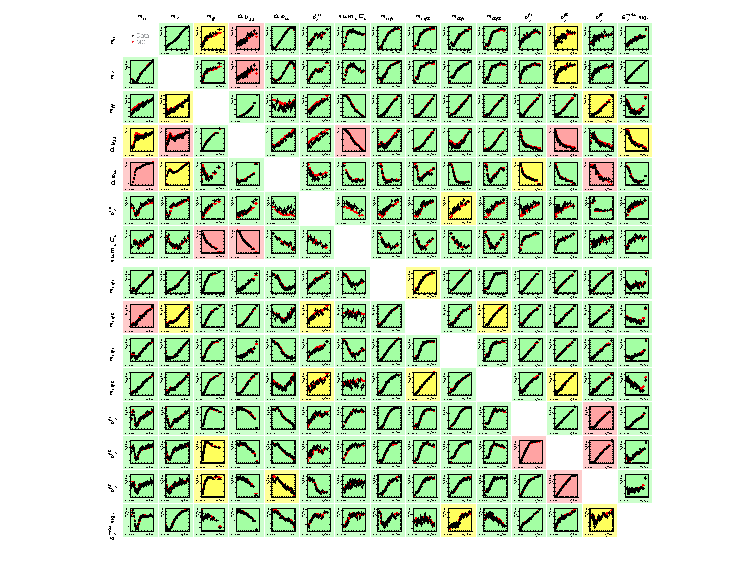
\includegraphics[width=\textwidth,trim=45 0 45 0]{figures/hww/dnn/correlations_PROF_SR.pdf}
    \caption{Visualization of the two-dimensional correlations between all combinations of DNN input variables, based on profiles of each of the distributions in the VBF-enriched \TwoJet SR. For all combinations of input variables $X_i$ and $X_j$, the distributions of both $\langle X_i \rangle$ vs $X_j$ and $\langle X_i \rangle$ vs $X_j$ are shown. The uncertainties are statistical only. The color for each plot encodes the $\chi^2$ probability, $p$, evaluated for each comparison: green represents $p > 0.05$, yellow represents $0.005 < p < 0.05$, and red represents $p < 0.005$.}
    \label{fig:dnn-features-profiles}
\end{figure}

\subsection{Construction and validation of final DNN discriminant}
\label{subsec:fina-model-validation}
Once the input variables are chosen and the hyperparameters are optimized, the DNN model can be deployed in the analysis. The test set is used for this purpose.
The binning of the DNN output is chosen based on a set of criteria.
The amount of VBF signal (background) events is required to be at least 20 (10) and the maximum allowed relative statistical uncertainty on the background expectation is 20\%.
These criteria ensure that there is sufficient statistical power in each bin in order to increase the robustness to statistical fluctuations and allow meaningful derivations of systematic uncertainties. At the same time, the binning is fine enough to exploit the shape of the VBF signal at high DNN output values.
The bins are found iteratively by moving the lower bound of a candidate bin to smaller values in steps of 0.01, starting with an upper bound at DNN output $= 1$. Once all criteria are met, a bin boundary is set and the lower bound is used as the new upper boundary for the next bin search. Even if the three criteria are fulfilled, no bin boundary is set if the VBF significance within a candidate bin is less than one third of the maximum significance of the bins already defined. This avoids a fine binning at low values of the DNN output where the signal sensitivity is limited.
The final DNN discriminant used in the statistical analysis is shown in \cref{sec:hww-results}, \cref{fig:VBF_DNN} with bin boundaries: [0-0.25, 0.25-0.52, 0.52-0.68, 0.68-0.77, 0.77-0.83, 0.83-0.87, 0.87-1.00].
For the STXS measurement, the statistical precision in the SRs is smaller. The binning criteria are therefore relaxed and only require at least 10 (5) signal (background) events. The requirement of the relative statistical uncertainty stays the same. In addition, the binning is harmonized between all 5 VBF STXS SRs, yielding bin boundaries: [0-0.5, 0.5, 0.74, 0.74-0.87, 0.87, 1.0]. The distributions are shown in \cref{sec:hww-results}, \cref{fig:aux:VBF-STXS-SRs}.

% \begin{figure}[th]
%     \centering
%     \newImageResizeCustom{0.6}{figures/220605-Thesis/sr/dnn-noDat/plots/run2-emme-CutVBF_SR-DNNoutputG_Fit-log.pdf}
%     {\caption{Distribution of the DNN output in the VBF SR with the final binning used in the statistical analysis.
%             \label{fig:dnn:blinded-fit-binning} }}
% \end{figure}
Before the data is analyzed in the signal sensitive range of the DNN, the modelling of the DNN output is validated in the CRs and VRs. This can be seen in \cref{fig:dnn:dnn-val-in-crs-a,fig:dnn:dnn-val-in-crs-b,fig:dnn:dnn-val-in-crs-c}. 
\begin{figure}[ht]
    \centering
    \subfloat[]{
        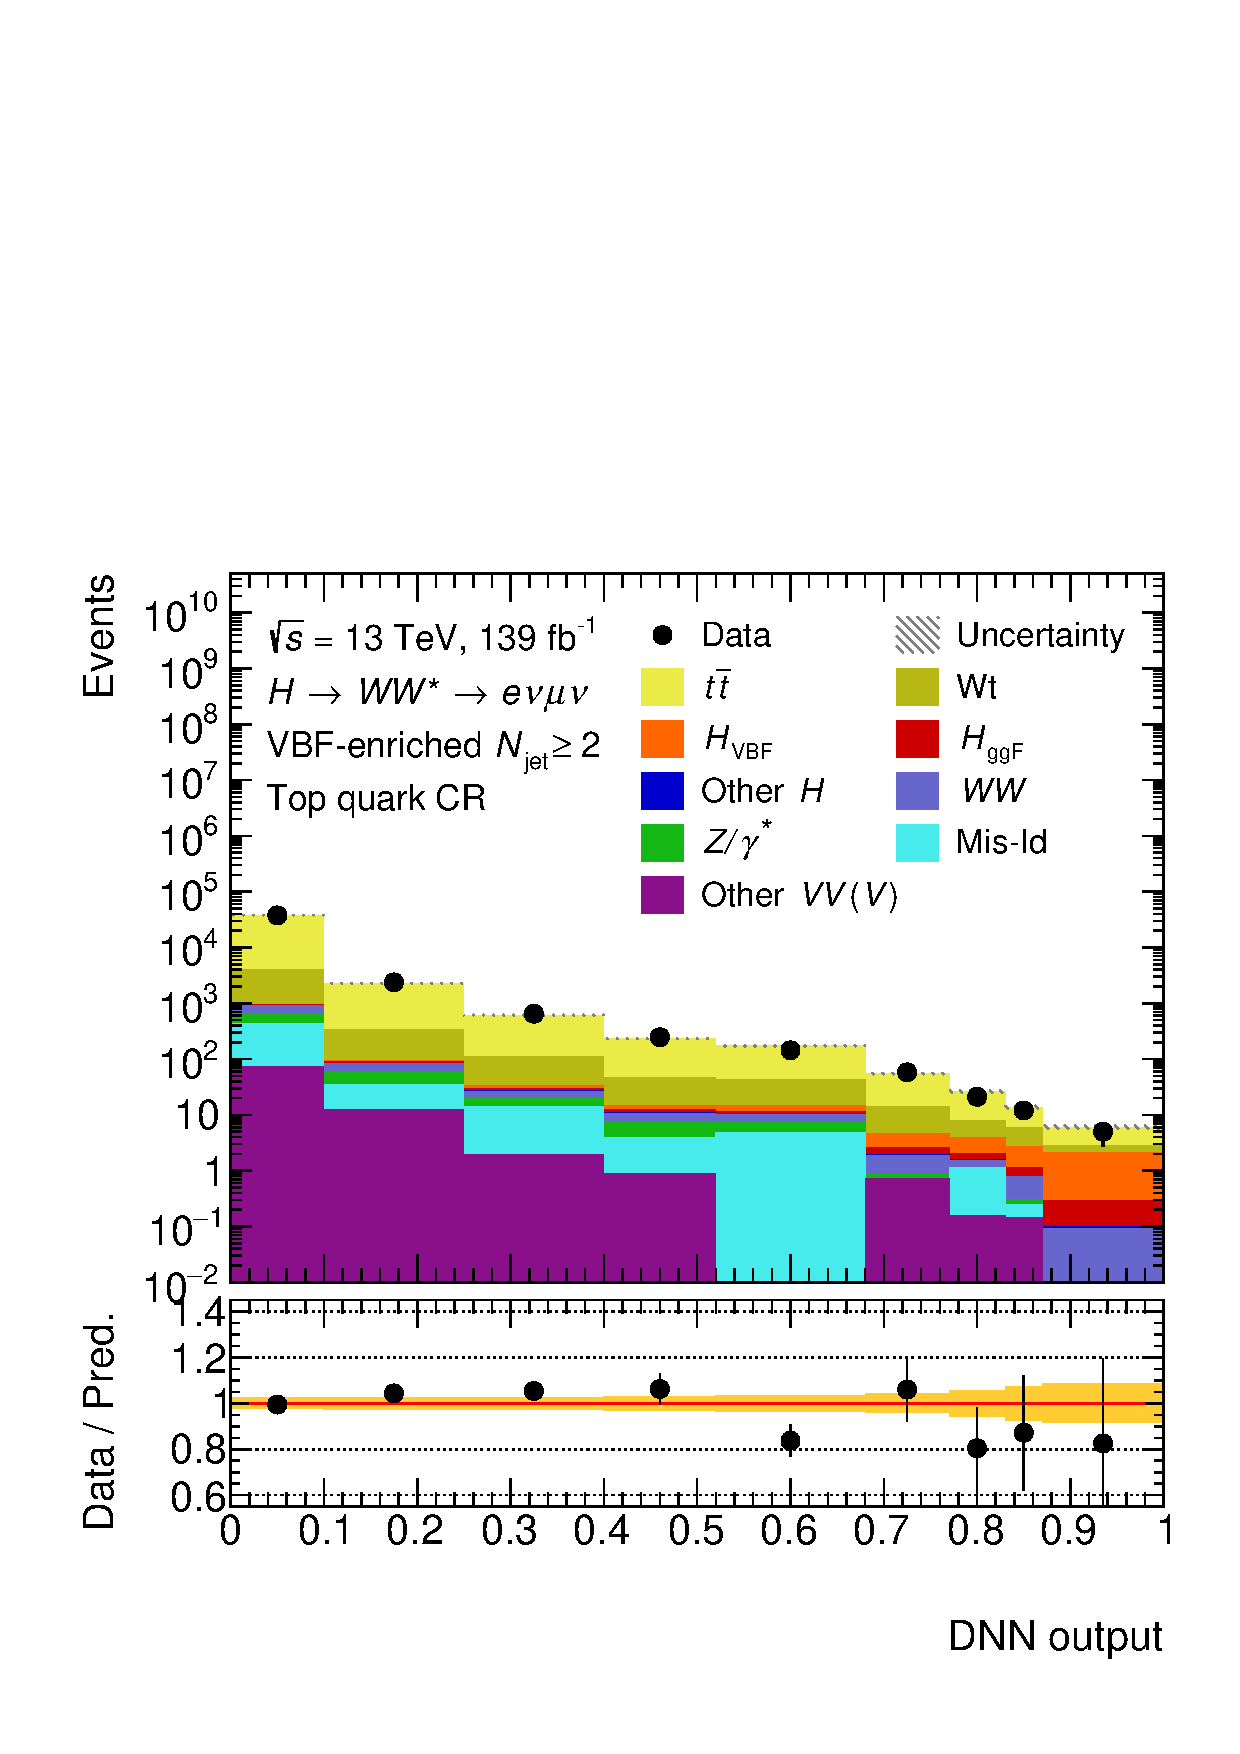
\includegraphics[width=0.47\textwidth]{figures/220605-Thesis/topcr/dnn/plots/run2-emme-CutVBF_TopControl_2jet-DNNoutputG_Fit_finelowDNN2-log}
        \label{fig:dnn:dnn-val-in-crs-a}
    }
    \subfloat[]{
        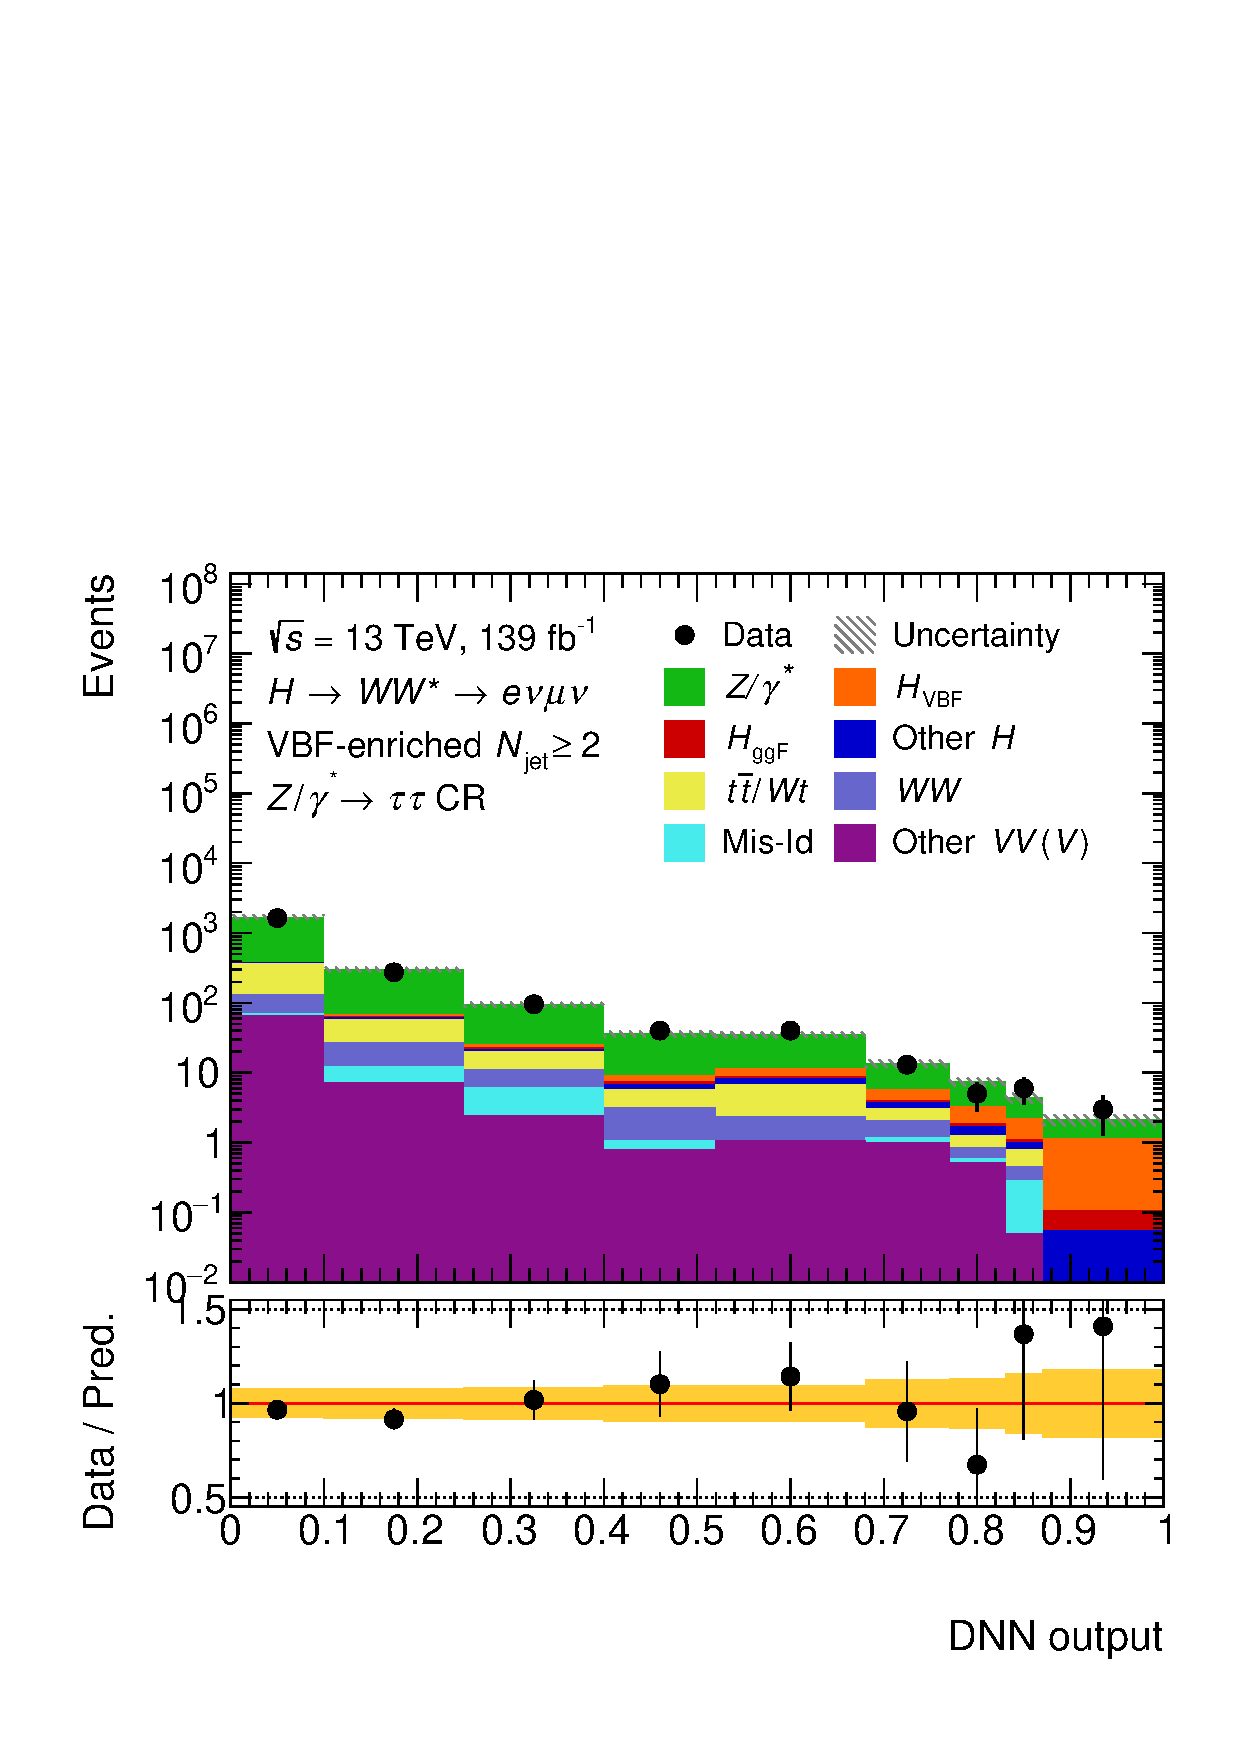
\includegraphics[width=0.47\textwidth]{figures/220605-Thesis/zttcr/dnn/plots/run2-emme-CutVBF_ZtautauControl_2jet-DNNoutputG_Fit_finelowDNN2-log}\hfill
        \label{fig:dnn:dnn-val-in-crs-b}
    }  \\
    \subfloat[]{
        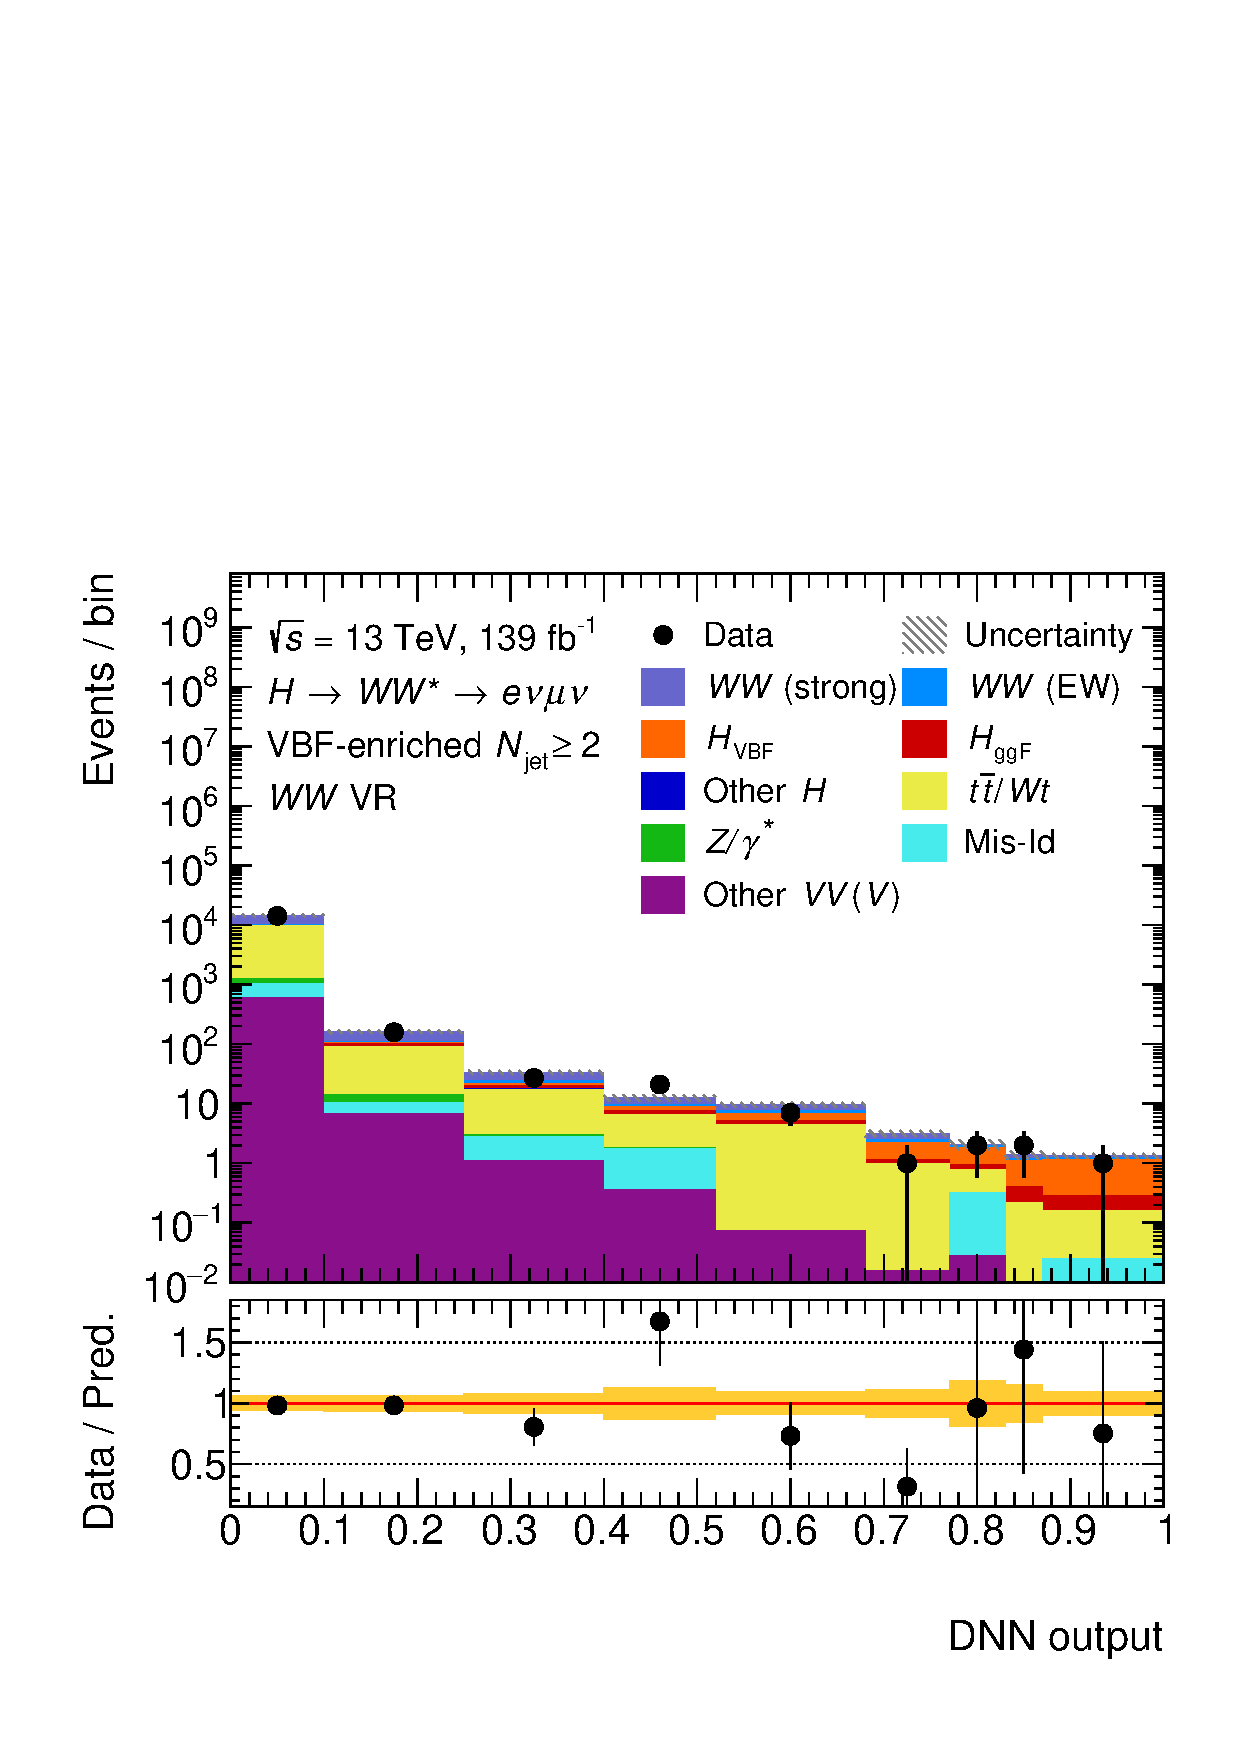
\includegraphics[width=0.47\textwidth]{figures/220605-Thesis/wwvr/dnn/plots/run2-emme-CutVBF_WWControl_2jet-DNNoutputG_Fit_finelowDNN2-log}
        \label{fig:dnn:dnn-val-in-crs-c}
    }
    \subfloat[]{
        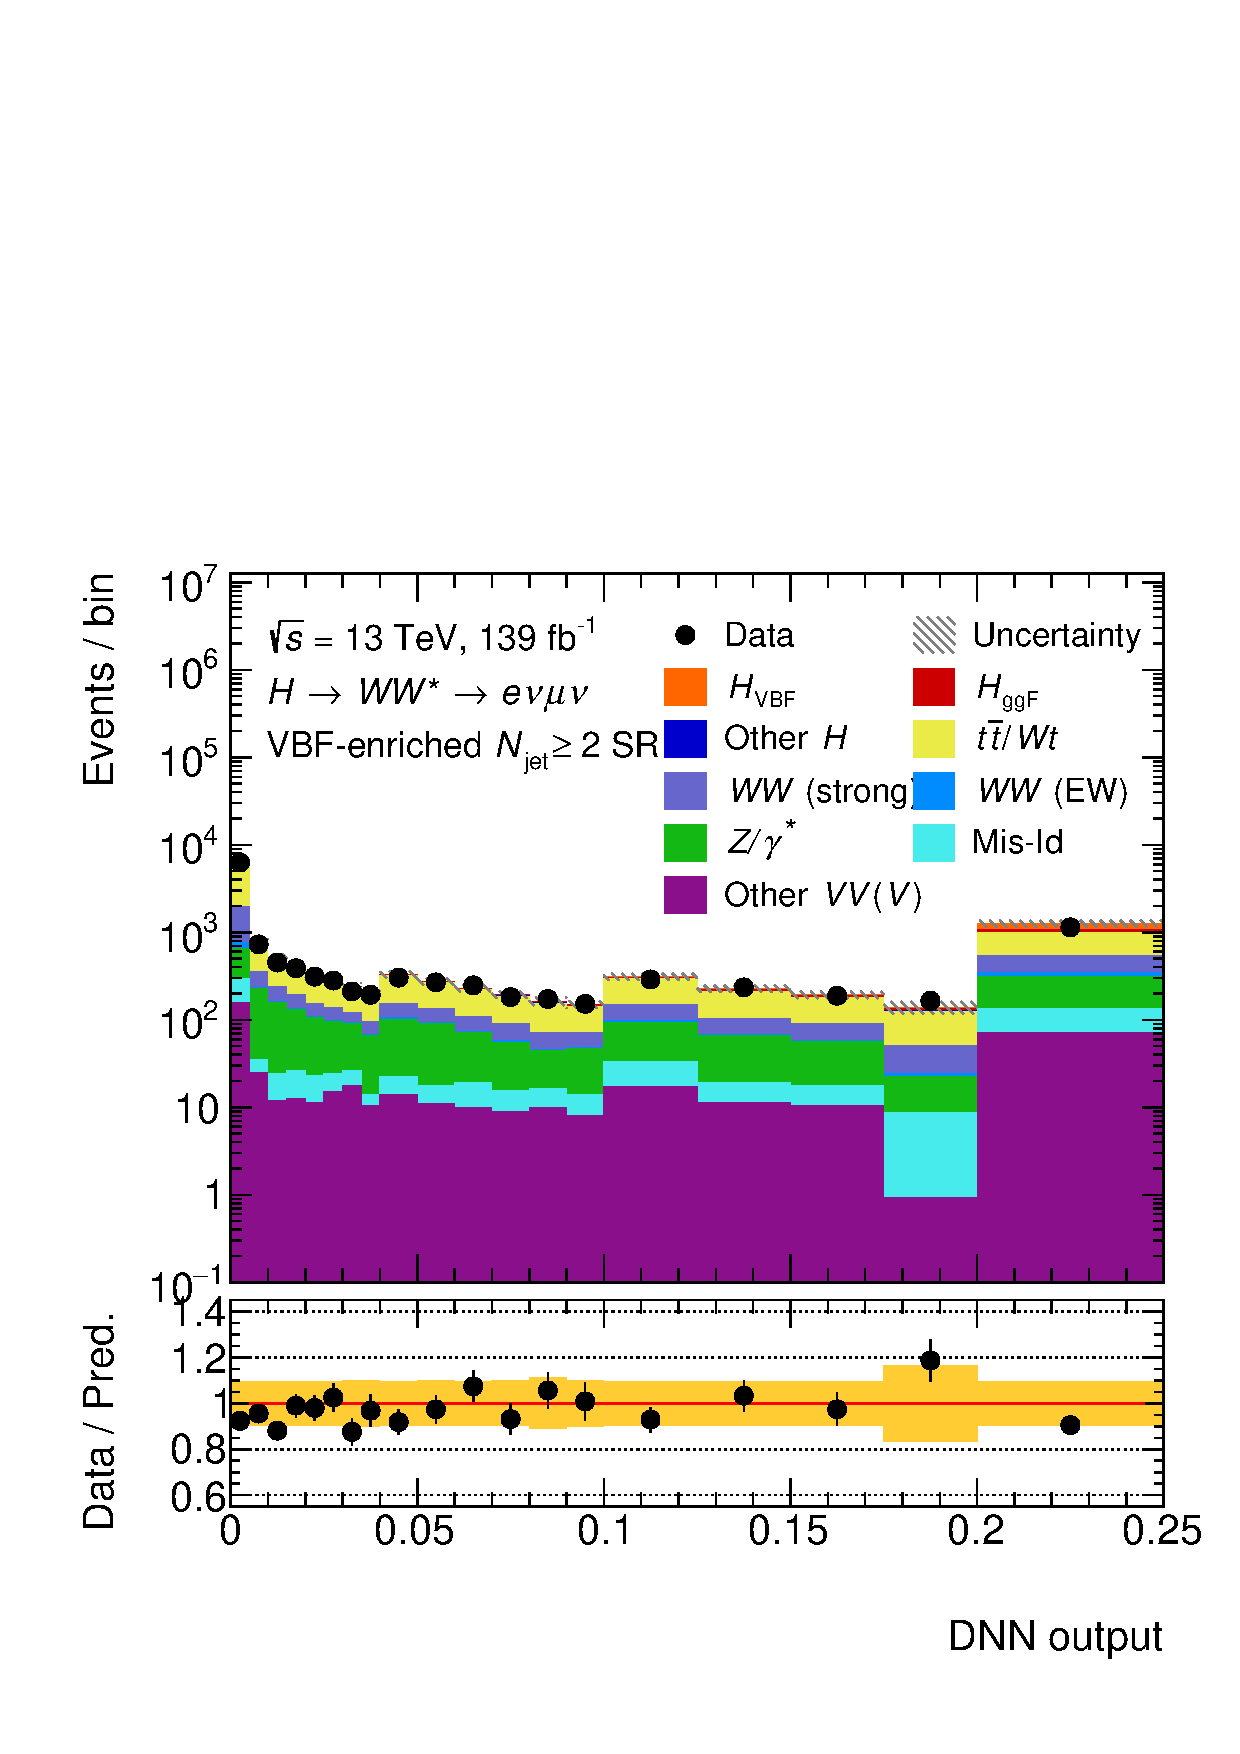
\includegraphics[width=0.47\textwidth]{figures/220605-Thesis/sr/dnn/plots/run2-emme-CutVBF_SR-DNNoutputG_blindRegion-log.pdf}
        \label{fig:dnn:dnn-val-in-crs-d}
    }
    {\caption{Distributions of the DNN output in (a) the top-quark CR, (b) the \Ztautau CR, (c) the $WW$ VR, and (d) the VBF SR with a requirement DNN output $<0.25$. The \Ztautau and top-quark processes are normalized using pre-fit normalization factors extracted from their corresponding CRs (NF$_{\Ztautau} = 1.00 \pm 0.04$, NF$_{\text{top}} = 1.00 \pm 0.01$). The yellow band corresponds to the square root of the sum in quadrature of the MC statistical uncertainties and the normalization component of the dominant experimental systematic uncertainties (JER, JES, Flavor-tagging, and \MET uncertainties). The various uncertainty components are discussed in more detail in \cref{sec:systematics}.
            \label{fig:dnn:dnn-val-in-crs} }}
\end{figure}
No evidence of significant discrepancy between the data and the MC simulation is found. In addition, the background-enriched region of the DNN output (DNN output $< 0.25$) can be validated in the VBF SR. \Cref{fig:dnn:dnn-val-in-crs-d} shows this region of the DNN output, binned finely to visualize potential differences.
Despite the small offset in the overall normalization, which is covered by the uncertainties, there is no significant sign of shape differences between the data and MC simulations.
A final cross-check is performed by studying the modelling of the input variables in the VBF SR with a selection made on the DNN output $< 0.25$ to avoid revealing the signal sensitive region. Representative distributions are shown in \cref{fig:srdnn25:dnn-inputs}.
Given the fact that only the normalization component and only a subset of systematic uncertainties are considered, they show acceptable consistency between data and MC simulation.
These validation studies establish the DNN output as a meaningful observable, so that it can be used as final discriminant in the statistical analysis.
More studies of the DNN observable and its input variables, in particular for the regions used in the STXS analysis, can be found in \cref{app:dnn:input-vars}.

\newcommand{\srdnnlowplotdir}{figures/220605-Thesis/sr/dnn25-scaledvbf-nfs3x3/plots}
\sixPlots{Distributions of (a) \mjj, (b) \dyjj, (c) \mlonejone, (d), \mll, (e) \lepetacent, and (f) \METSig in the VBF SR selecting only the region below DNN output $= 0.25$. The solid orange line shows the expected VBF signal scaled by a factor of 200. The \Ztautau and top-quark processes are normalized using pre-fit normalization factors extracted from their corresponding CRs (NF$_{\Ztautau} = 1.01 \pm 0.04$, NF$_{\text{top}} = 1.00 \pm 0.01$). The last bin of the distributions include the overflow. The yellow band corresponds to the square root of the sum in quadrature of the MC statistical uncertainties and the normalization component of the dominant experimental systematic uncertainties (JER, JES, Flavor-tagging, and \MET uncertainties). The various uncertainty components are discussed in more detail in \cref{sec:systematics}.
}{fig:srdnn25:dnn-inputs}{\srdnnlowplotdir/run2-emme-CutVBFSR_25DNN-Mjj-log.pdf}{\srdnnlowplotdir/run2-emme-CutVBFSR_25DNN-DYjj-lin.pdf}{\srdnnlowplotdir/run2-emme-CutVBFSR_25DNN-DPhill-lin.pdf}{\srdnnlowplotdir/run2-emme-CutVBFSR_25DNN-Mll-lin.pdf}{\srdnnlowplotdir/../../dnn25-scaledvbf-lepcent-nfs3x3/plots/run2-emme-CutVBFSR_25DNN-contOLV-lin.pdf}{\srdnnlowplotdir/run2-emme-CutVBFSR_25DNN-METSig_broad-lin.pdf}

